% ========================================= TEMPLATE INFO ========================================
%
% Author:       P4ntomime
% Version:      1.0.0
% Last updated: 2024-02-18
% Brief:        A LaTeX template for summaries. See README.md for more information.
% 
% ================================================================================================
\documentclass[8pt, a4paper, twoside]{extarticle}
% Font size:    8pt
% Paper size:   A4
% style:        twoside (needed, so odd and even pages have different margins)
% orientation:  portrait. (use 'landscape' for landscape orientation)


% ========================================= DOCUMENT INFO =========================================
\def\title{Embedded Software Engineering 1}           % title
\def\shorttitle{EmbSW1}     % short title (displayed as PDF title)
\def\dozent{Prof. Reto Bonderer}  % lecturer
\def\semester{HS 2024}      % semester
\def\author{Laurin Heitzer, Simone Stitz}        % author(s)
\def\repo{https://github.com/P4ntomime/EmbSW1}   % repository link
\def\version{1.0.\today}    % version
\def\pagelimit{20}          % page limit -> causes pages after limit to be red
\def\titleoption{compact}   % options: compact, normal
\def\enableToC{true}

% ================================= PACKAGES, SETUP AND COMMANDS ==================================
% =========================================== PACKAGES ============================================
\usepackage[utf8]{inputenc}         % input encoding: UTF-8
\usepackage[T1]{fontenc}            % font encoding: T1
\usepackage{textcomp}               % additional symbols
\usepackage{times}                  % times new roman font
\usepackage{inconsolata}            % use consolas font for ttfamily
\usepackage[main=ngerman]{babel}    % set main language to german


\usepackage{multicol}               % provides multicols environment
\usepackage{geometry}               % set page layout


\usepackage{enumitem}               % list customization
\usepackage{outlines}               % easy nested lists
\usepackage{tabularx}               % some nicer tables with X columns
\usepackage{hhline}                 % double lines in tables
\usepackage{booktabs}               % thick and thin lines in tables
\usepackage{boldline}               % bold (vertical) lines in tables


\usepackage{amsmath}                % math symbols
\usepackage{amssymb}                % more math symbols
\usepackage{mathtools}              % more math tools needed for pmatrix modification
\usepackage{mhsetup}                % needed to modify pmatrix environment
\usepackage{txfonts}                % Times math font
\usepackage[squaren]{SIunits}       % SI-units
\usepackage{bm}                     % bold math symbols
\usepackage{trfsigns}               % needed for "Laplace" symbol (Korrespondenz)
\usepackage{mathrsfs}               % needed for Fourier transform "F"


\usepackage{graphicx}               % include graphics
\usepackage{graphbox}               % needed for aligning images in multicol environment
\usepackage{scalerel}               % scale any objects
\usepackage{anyfontsize}            % set any font size
\usepackage[table]{xcolor}          % needed for colors


\usepackage{tcolorbox}              % colored boxes
\usepackage[outline]{contour}       % contour for text (used in custom underline command)
\usepackage[normalem]{ulem}         % custom underline (used in custom underline command)


\usepackage{tikz}                   % needed for TikZ drawings

\usepackage{pgfplots}               % needed for  easy axis generation in TikZ drawings
\pgfplotsset{compat=1.17}	        % newest version
\AtBeginEnvironment{tikzpicture}{\tracinglostchars=0\relax}

\usepackage{listings}               % for nicer code display
% to use nodes inside listing see: https://texample.net/tikz/examples/tikz-listings/


\usepackage{hyperref}               % clickable links
\usepackage{qrcode}                 % QR code generation (also clickable)


\usepackage{ifthen}                 % if-then-else commands
\usepackage{calc}                   % simple arithmetic in LaTeX commands


\usepackage{draftwatermark}         % watermark on pages after a certain limit
\usepackage{fancyhdr}               % custom header and footer
\usepackage[explicit]{titlesec}     % custom section titles


\usepackage{datetime2}              % custom date format for versioning


% ========================================== BASIC SETUP ==========================================

% --------------------------------------- DOCUMENT SETTINGS ---------------------------------------
\hypersetup{hidelinks,
% set pdf metadata
            pdfauthor={\author},
            pdftitle={\shorttitle},
            pdfsubject={\title\ \semester},
            pdfkeywords={Gahn go lerne!!}}

% set style for URLs
\urlstyle{same} % sets url font to the same as the preceeding text

% set page layout
\geometry{left=3mm, 
          right=3mm, 
          top=3mm, 
          bottom=6mm, 
          headheight=0mm, 
          headsep=0mm, 
          footskip=4mm}

\setlength{\columnsep}{1.5mm}       % distance between columns
\setlength{\columnseprule}{0.1pt}   % thickness of column separation line
\setlength{\parindent}{0pt}         % no paragraph indentation

\setcounter{tocdepth}{2}            % only display sections and subsections in toc
% \setcounter{secnumdepth}{0}       % uncomment to disable section numbering

\DeclareMathSizes{8}{8}{6}{5}       % set math font sizes for 8pt document


% --------------------------------------- COLOR DEFINITIONS ---------------------------------------
\definecolor{sectioncolor}{HTML}{1ef943}
\definecolor{subsectioncolor}{HTML}{a4fdb4}
\definecolor{sectextcol}{HTML}{000000}
\definecolor{subsectextcol}{HTML}{000000}

\definecolor{backcolour}{HTML}{f5f5f0} % background color for highlighted text

% TODO: define color palette
% color palette: https://colorkit.co/color-palette-generator/FF8552-9e22bd-404E7C-C32E15-225A28/
\definecolor{green}{HTML}{1af430}
\definecolor{red}{HTML}{f90d09}
\definecolor{blue}{HTML}{093ce5}
\definecolor{orange}{HTML}{f7730e}
\definecolor{violet}{HTML}{a516c9}

% colors for listings (code)
\definecolor{commentcolour}{HTML}{008000}
\definecolor{keywordcolour}{HTML}{7f0055}
\definecolor{stringcolour}{HTML}{9e22bd}
\definecolor{numbercolour}{HTML}{808080}
% \definecolor{commentcolour}{HTML}{404E7C}
% \definecolor{keywordcolour}{HTML}{225A28}
% \definecolor{stringcolour}{HTML}{9e22bd}
% \definecolor{numbercolour}{HTML}{808080}
% colors for listings (code) according to ProgCPP
\definecolor{codeblue}{RGB}{2, 90, 200}
\definecolor{codegreen}{rgb}{0,0.6,0}
\definecolor{codegray}{rgb}{0.5,0.5,0.5}
\definecolor{codepurple}{rgb}{0.58,0,0.82}
\definecolor{backcolour}{rgb}{0.95,0.95,0.92}


% ----------------------------------- LIST AND TABULAR SETTINGS -----------------------------------
\setlist[enumerate]{%
    labelindent=0pt,                                % no indentation for labels
    labelwidth = \widthof{\ref{enum-\EnumitemId}},  % set label width to widest label
    label=\bfseries\arabic*.,                       % label style bold arabic numerals (1., 2., ...)
    itemindent=1ex,                                 % separation between label and item text
    leftmargin=!,                                   % automatically calculate left margin
    after=\label{enum-\EnumitemId}}                 % set label for referencing in labelwidth

\setlist[description]{leftmargin=2ex}               % left margin for description: 2ex
\setlist[itemize]{leftmargin=1.5em}                 % left margin for itemize: 1.5em
\setlist[description]{leftmargin=2ex}               % left margin for description: 2ex
\setlist{nosep}                                     % no vertical spacing between list items

\renewcommand{\arraystretch}{1}                     % stretch table rows

\setcounter{MaxMatrixCols}{32}                      % increase max columns in matrix environments

% ----------------------------------------- TIKZ SETTINGS -----------------------------------------
\usetikzlibrary{arrows}
\usetikzlibrary{arrows.meta}
\usetikzlibrary{bending}
\usetikzlibrary{decorations.pathreplacing}
\usetikzlibrary{angles}
\usetikzlibrary{tikzmark}
\usetikzlibrary{petri}
\usetikzlibrary{positioning}
\usetikzlibrary{shapes}
\usetikzlibrary{calc}


% ------------------------------------ OTHER PACKAGE SETTINGS -------------------------------------

% define and set new date style for versioning as YYYYMMDD
\DTMnewdatestyle{vnumdate}{%
    \renewcommand{\DTMdisplaydate}[4]{\number##1\DTMtwodigits{##2}\DTMtwodigits{##3}}%
    \renewcommand{\DTMDisplaydate}{\DTMdisplaydate}%
}
\DTMsetdatestyle{vnumdate}


% setup for ulem and contour packages
\renewcommand{\ULdepth}{1.75pt} % set underline depth
\contourlength{0.7pt}           % set contour length


% ====================================== SETUP AND COMMANDS =======================================

% custom font size for paragraph titles
\newcommand{\semilarge}{\fontsize{9}{8}\selectfont} % new font size \semilarge (9pt)

\ExplSyntaxOn
% custom underline command for exclusions on lowercase letters such as g, j, p, q, y
\newrobustcmd{\myul}[1]{%
    \if_mode_math:
        \text{%
            \uline{\phantom{$#1$}}%
            \llap{\contour{white}{$#1$}}%
        }
    \else:
        \uline{\phantom{#1}}%
        \llap{\contour{white}{#1}}%
    \fi:
}

\renewrobustcmd{\underline}[1]{%
    \if_mode_math:
        \text{%
            \uline{\phantom{$#1$}}%
            \llap{\contour{white}{$#1$}}%
        }
    \else:
        \uline{\phantom{#1}}%
        \llap{\contour{white}{#1}}%
    \fi:
}
\ExplSyntaxOff


% setup header and footer
\pagestyle{fancy}
\fancyhf{}                          % clear all header and footer fields
\renewcommand{\headrulewidth}{0pt}  % remove header rule
\renewcommand{\footrulewidth}{0pt}  % remove footer rule
\fancyfoot[C]{\thepage}             % page number in center of footer


% --------------------------------------- TITLE FORMATTING ----------------------------------------

% section formatting
\titleformat{\section}
            % {\fontsize{9}{8}\selectfont\bfseries}
            {\Large\bfseries}
            {}
            {0mm}
            {\tikz{
                \node[fill=sectioncolor,            % fill color:       sectioncolor
                      text=sectextcol,              % text color:       sectextcol
                      text width=\columnwidth-4pt,  % text width:       columnwidth - 2x padding
                      text depth=0pt,               % text depth:       0pt (needed so text stays vertically centered)
                      minimum height=5mm,           % minimum height:   5mm
                      inner sep=2pt,                % inner padding:    2pt
                      align=left]                   % text alignment:   left
                      {\thesection\ #1};}}

\titleformat{numberless, name=\section}
            % {\fontsize{9}{8}\selectfont\bfseries}
            {\Large\bfseries}
            {}
            {0mm}
            {\tikz{
                \node[fill=sectioncolor,            % fill color:       sectioncolor
                      text=sectextcol,              % text color:       sectextcol
                      text width=\columnwidth-4pt,  % text width:       columnwidth - 2x padding
                      text depth=0pt,               % text depth:       0pt (needed so text stays vertically centered)
                      minimum height=5mm,           % minimum height:   5mm
                      inner sep=2pt,                % inner padding:    2pt
                      align=left]                   % text alignment:   left
                      {#1};}}

\titlespacing{\section}
             {0mm}
             {.2ex}
             {.2ex}


% subsection formatting
\titleformat{\subsection}
            {\large\bfseries}
            {}
            {0mm}
            {\phantomsection\tikz{
                \node[fill=subsectioncolor,         % fill color:       subsectioncolor 
                      text=subsectextcol,           % text color:       subsectextcol 
                      text width=\columnwidth-4pt,  % text width:       columnwidth - 2x padding 
                      text depth=0pt,               % text depth:       0pt (needed so text stays vertically centered)
                      minimum height=5mm,           % minimum height:   5mm 
                      inner sep=2pt,                % inner padding:    2pt 
                      align=left]                   % text alignment:   left
                      {\thesubsection\ #1};}}

\titleformat{numberless, name=\subsection}
            {\large\bfseries}
            {}
            {0mm}
            {\phantomsection\tikz{
                \node[fill=subsectioncolor,         % fill color:       subsectioncolor 
                      text=subsectextcol,           % text color:       subsectextcol 
                      text width=\columnwidth-4pt,  % text width:       columnwidth - 2x padding 
                      minimum height=5mm,           % minimum height:   5mm 
                      inner sep=2pt,                % inner padding:    2pt 
                      align=left]                   % text alignment:   left
                      {#1};}}

\titlespacing{\subsection}
             {0mm}
             {1ex}
             {.2ex}


% subsubsection formatting
\titleformat{\subsubsection}
            {\large\bfseries}
            {\myul{\thesubsubsection\ }}
            {0mm}
            {\phantomsection{}\myul{#1}}

\titlespacing{\subsubsection}
             {0mm}
             {1ex}
             {1ex}


% paragraph formatting
\titleformat{\paragraph}[hang]
            {\semilarge\bfseries}
            {}
            {0mm}
            {#1\normalfont :\;}

\titlespacing{\paragraph}
             {0mm}
             {1.5ex}
             {0.1ex}


% new alias for paragraph '\para' (shorter than \paragraph)
\let\para\paragraph%

% custom command for examples
\newcommand{\example}[1]{\subsubsection*{Beispiel: #1}}


% ----------------------------------- CUSTOM TABULAR SPECIFIERS -----------------------------------

% centered fixed width column type
\newcolumntype{P}[1]{>{\centering\arraybackslash}p{#1}}

 % centered variable width column type
\newcolumntype{C}{>{\centering\arraybackslash}X}

% centered math column type
\newcolumntype{M}{>{$}c<{$}}


% inline tikz node for later referencing
\newcommand{\tikznode}[2]{% from https://tex.stackexchange.com/a/402466/121799
	\ifmmode%
	\tikz[remember picture,baseline= (#1.base),inner sep=0pt] \node(#1){$#2$};
	\else
	\tikz[remember picture,baseline= (#1.base),inner sep=0pt] \node(#1){#2};
	\fi}


% custom inline tcolorbox
\newtcbox{\mybox}
            [1]
            [backcolour]
            {on line,
            arc=0pt,
            outer arc=0pt,
            colback=#1,
            colframe=#1,
            boxsep=0pt,
            left=1pt,
            right=1pt,
            top=1pt,
            bottom=1pt,
            boxrule=0pt}


\makeatletter

% ------------------------------- SECTIONING COMMANDS CUSTOMIZATION -------------------------------

% section: add optional argument to command for script page numbers
\let\old@sec\section%
\RenewDocumentCommand{\section}{somg}{%
    \IfBooleanTF{#1}{
        \IfNoValueTF{#2}{
            \IfNoValueTF{#4}{
                \old@sec*{#3}
            }{
                \old@sec*{#3 {\small(S. #4)}}
            }
        }{
            \IfNoValueTF{#4}{
                \old@sec*[#2]{#3}
            }{
                \old@sec*[#2]{#3 {\small(S. #4)}}
            }
        }%
    }{
        \IfNoValueTF{#2}{
            \IfNoValueTF{#4}{
                \old@sec{#3}
            }{
                \old@sec{#3 {\small(S. #4)}}
            }
        }{
            \IfNoValueTF{#4}{
                \old@sec[#2]{#3}
            }{
                \old@sec[#2]{#3 {\small(S. #4)}}
            }
        }%
    }
}


% subsection: add optional argument to command for script page numbers
\let\old@subsec\subsection%
\RenewDocumentCommand{\subsection}{somg}{%
    \IfBooleanTF{#1}{
        \IfNoValueTF{#2}{
            \IfNoValueTF{#4}{
                \old@subsec*{#3}
            }{
                \old@subsec*{#3 {\small(S. #4)}}
            }
        }{
            \IfNoValueTF{#4}{
                \old@subsec*[#2]{#3}
            }{
                \old@subsec*[#2]{#3 {\small(S. #4)}}
            }
        }%
    }{
        \IfNoValueTF{#2}{
            \IfNoValueTF{#4}{
                \old@subsec{#3}
            }{
                \old@subsec{#3 {\small(S. #4)}}
            }
        }{
            \IfNoValueTF{#4}{
                \old@subsec[#2]{#3}
            }{
                \old@subsec[#2]{#3 {\small(S. #4)}}
            }
        }%
    }
}


% subsubsection: add optional argument to command for script page numbers
\let\old@subsubsec\subsubsection%
\RenewDocumentCommand{\subsubsection}{somg}{%
    \IfBooleanTF{#1}{
        \IfNoValueTF{#2}{
            \IfNoValueTF{#4}{
                \old@subsubsec*{#3}
            }{
                \old@subsubsec*{#3 {\small(S. #4)}}
            }
        }{
            \IfNoValueTF{#4}{
                \old@subsubsec*[#2]{#3}
            }{
                \old@subsubsec*[#2]{#3 {\small(S. #4)}}
            }
        }%
    }{
        \IfNoValueTF{#2}{
            \IfNoValueTF{#4}{
                \old@subsubsec{#3}
            }{
                \old@subsubsec{#3 {\small(S. #4)}}
            }
        }{
            \IfNoValueTF{#4}{
                \old@subsubsec[#2]{#3}
            }{
                \old@subsubsec[#2]{#3 {\small(S. #4)}}
            }
        }%
    }
}


% custom text rightarrow to match tikz arrows
\renewrobustcmd{\textrightarrow}{%
    \raisebox{0.2ex}{%
        \tikz[line width=0.11ex, >={Stealth[length=1.1ex, inset=0.2ex]}]{%
            \draw (0,-0.13ex) to (0.55em, -0.13ex);%
            \draw (0, 0.13ex) to (0.55em,  0.13ex);%
            \draw[line width=0pt, ->] (0.8em,0) to (0.9em,0);%
        }%
    }%
}%

% custom text leftrightarrow to match tikz arrows
\newrobustcmd{\textlrarrow}{%
    \raisebox{0.2ex}{%
        \tikz[line width=0.11ex, >={Stealth[length=1.1ex, inset=0.2ex]}]{%
            \draw (0.35em,-0.13ex) to (0.9em, -0.13ex);%
            \draw (0.35em, 0.13ex) to (0.9em,  0.13ex);%
            \draw[line width=0pt, ->] (1.15em,0) to (1.25em,0);%
            \draw[line width=0pt, <-] (0,0) to (0.1em,0);%
        }%
    }%
}%


% renews the pmatrix environment to use \lgroup and \rgroup instead of \left( and \right)
\renewenvironment{pmatrix}{%
    \left\lgroup%
    \matrix@check\pmatrix\env@matrix%
}{
    \endmatrix\right\rgroup%
}

% renews the pmatrix* environment to use \lgroup and \rgroup instead of \left( and \right)
\MHInternalSyntaxOn%
\renewenvironment{pmatrix*}[1][c]
  {\left\lgroup\MT_matrix_begin:N #1}
  {\MT_matrix_end:\right\rgroup}
\MHInternalSyntaxOff%


% new environment for centered tabulars
\NewDocumentEnvironment{ctabular}{m}
                        {\center\tabular{#1}}
                        {\endtabular\endcenter}


% custom command for size matched colored brackets
\newcommand{\bbr}[2]{\colorlet{saved}{.}\color{#1}\left(\color{saved}#2\color{#1}\right)\color{saved}}


% custom command for differential operator d
\newcommand{\diff}{\ensuremath{\mathop{} \! \mathrm{d}}}

% custom command for underset limes operator
\newcommand{\limes}[1]{\ensuremath{\underset{#1}{\lim}}}

% custom command for absolute value
\newcommand{\abs}[1]{\ensuremath{\left|#1\right|}}


% shortcuts for colored text
\newcommand{\cgn}[1]{{\color{green}#1}}
\newcommand{\crd}[1]{{\color{red}#1}}
\newcommand{\cbl}[1]{{\color{blue}#1}}
\newcommand{\cor}[1]{{\color{orange}#1}}
\newcommand{\cvt}[1]{{\color{violet}#1}}



% bullet command for items in tables
\newcommand{\tabitem}{~~\llap{\textbullet}~~}


% customizes watermark and page color after a certain page limit
% colors all pages after the specified limit red
% source: https://stackoverflow.com/questions/2720534/force-a-maximum-number-of-pages-in-latex 
\newcounter{page@count}
\setcounter{page@count}{0}
\gdef\maxpages{\pagelimit}
\ifx\latex@outputpage\@undefined\relax% ChkTeX 21
    \global\let\latex@outputpage\@outputpage% ChkTeX 21
\fi%
\gdef\@outputpage{% ChkTeX 21
    \addtocounter{page@count}{1}%
    \ifnum\value{page@count}>\maxpages\relax%
        % change page background to red and add watermark
        \SetWatermarkText{\pagelimit\ Seiten Limit erreicht!}%
        \SetWatermarkScale{0.35}%
        \pagecolor{red}
        \latex@outputpage%
    \else%
        \SetWatermarkText{}%
        \latex@outputpage%
    \fi%
}


% remove title from table of contents, needed for layout
\renewcommand{\tableofcontents}{%
    \@starttoc{toc}
}


% scale super- and subscript -- not used currently, instead resized math font
% \catcode`_=\active% chktex 41 --> suppress ChkTeX warning
% \catcode`^=\active% chktex 41
% \newcommand_[1]{\ensuremath{\sb{\mathrm{\scaleobj{0.7}{#1}}}}}
% \newcommand^[1]{\ensuremath{\sp{\mathrm{\scaleobj{0.7}{#1}}}}}


\makeatother


% new environment for layout --> automatically adjusts to landscape or portrait
\ExplSyntaxOn
\NewDocumentEnvironment{layout}{}{
    \dim_compare:nNnT{\paperwidth}<{\paperheight}
    {
        % PORTRAIT LAYOUT
        \str_case:en{\str_lowercase:f\titleoption}
        {
            {compact}
            {
                \str_if_eq:eeTF {\str_lowercase:f\enableToC}{true}
                {
                    \begin{minipage}[t]{0.1\columnwidth} % Elo-like formatting
                        \raisebox{-.3\columnwidth}{\qrcode[level=L, 
                                version=0,
                                height=0.9\columnwidth]{\repo}}\\[1mm]
                        \normalfont\footnotesize V \version{}
                        \smallskip
                    \end{minipage}\hfill
                    \begin{minipage}[t]{0.89\columnwidth}
                        \raggedright%
                        \normalfont\Huge\bfseries\title{}\\[1mm]
                        \normalfont\Large\semester\ --\ \dozent{}\\
                        \large Autoren:\ \author{}\\[1mm]
                        \myul{\url{\repo}}
                    \end{minipage}\par
                    \section*{\contentsname}
                    \group_begin:
                    \setlength{\columnsep}{5mm}
                    \begin{multicols}{2}
                        \tableofcontents%
                    \end{multicols}
                    \group_end:
                    \vfill
                    \newpage
                    \begin{multicols*}{2}
                    \raggedcolumns%
                }
                {
                    \begin{multicols*}{2}
                    \raggedcolumns%
                    \begin{minipage}[t]{0.2\columnwidth} % MathFML-like formatting
                        \vspace{-0.225\columnwidth}
                        \qrcode[level=L, 
                                version=0,
                                height=0.9\columnwidth]{\repo}\\[1mm]
                        \normalfont\footnotesize V \version{}
                        \smallskip
                    \end{minipage}\hfill
                    \begin{minipage}[t]{0.79\columnwidth}
                        \raggedright%
                        \normalfont\Huge\bfseries\title{}\\[1mm]
                        \normalfont\Large\semester\ --\ \dozent{}\\
                        \large Autoren:\ \author{}\\[1mm]
                        \normalsize\myul{\url{\repo}}
                    \end{minipage}\par
                }
            }
            {normal}
            {
                \hfill\null\vspace{1cm}
                \begin{center}
                    \normalfont\fontsize{35}{32}\selectfont\bfseries\title{}\\[7.5mm]
                    \normalfont\huge\semester\ --\ \dozent{}\\
                    \Large Autoren:\\
                    \Large\author{}\\[2mm]
                    \large Version:\\
                    \large\version{}\\
                    \normalsize\myul{\url{\repo}}\\[2mm]
                    \qrcode[level=L, 
                            version=0,
                            height=2cm]{\repo}
                \end{center}
                \vfill
                \thispagestyle{empty}
                \str_if_eq:eeT {\str_lowercase:f\enableToC}{true}
                {
                    \section*{\contentsname}
                    \group_begin:
                    \setlength{\columnsep}{5mm}
                    \begin{multicols}{2}
                        \tableofcontents%
                    \end{multicols}
                    \group_end:
                    \vfill
                }
                \newpage
                \begin{multicols*}{2}
                \raggedcolumns%
            }
        }
    }
    
    \dim_compare:nNnT{\paperwidth}>{\paperheight}
    {
        % LANDSCAPE LAYOUT
        \begin{multicols*}{3}
        \raggedcolumns%            
        \begin{minipage}[t]{0.18\columnwidth}
            \vspace{-0.225\columnwidth}
            \qrcode[level=L, 
                    version=0,
                    height=0.9\columnwidth]{\repo}\\[1mm]
            \normalfont\footnotesize V \version{}
            \smallskip
        \end{minipage}\hfill
        \begin{minipage}[t]{0.81\columnwidth}
            \raggedright%
            \normalfont\Huge\bfseries\title{}\\
            \normalfont\Large\semester\ --\ \dozent{}\\
            \large Autoren:\ \author{}\\
            \normalsize\myul{\url{\repo}}
        \end{minipage}\par % \par needed or else there is an underfull hbox warning
        \str_if_eq:eeT {\str_lowercase:f\enableToC}{true}
        {
            \section*{\contentsname}
            \resizebox{\columnwidth}{!}{%
                \begin{minipage}[t]{1.2\columnwidth}
                    \begin{multicols}{2}
                        \tableofcontents%
                    \end{multicols}
                \end{minipage}
            }\par
        }
    }%
}
{\end{multicols*}}
\ExplSyntaxOff

% ---------------------------------------- LISTINGS SETUP -----------------------------------------

% hack to fix asterisk in lstlisting
\makeatletter
\lst@CCPutMacro%
    \lst@ProcessOther{"2A}{% ChkTeX 18
         {\raisebox{0.125pt}{*}}}
    \@empty\z@\@empty% ChkTeX 21
\makeatother


% inline lst tikz node for later referencing
\newcommand{\lstnode}[2][0.5ex]{
	\tikz[overlay, remember picture, inner sep=0pt, yshift=#1, minimum width=0mm]\node(#2){};
}


% custom inline listings with box around them
\newcommand{\mylstbox}[2][columns=fullflexible]{%
    \mybox{%
        \lstinline[#1]{#2}}}
\newcommand{\mytclstbox}[2][black]{%
    \mybox{%
        \lstinline[basicstyle=\sffamily\footnotesize\color{#1}, columns=fullflexible]{#2}}}


% % renew command for lstinputlisting with less vertical spacing
% \renewcommand{\lstinputlisting}[2][]{
%     \begingroup
%     \vspace{-0.6\abovedisplayskip}
%     \lst@setcatcodes%
%     \lst@inputlisting[#1]{#2}
%     \vspace{-0.6\abovedisplayskip}
% }

% listings style (code)
% \lstdefinestyle{mystyle}{
%     backgroundcolor=\color{backcolour},   
%     commentstyle=\color{codegreen},
%     keywordstyle=\color{codeblue},
%     numberstyle=\tiny\color{codegray},
%     stringstyle=\color{codepurple},
%     basicstyle=\ttfamily\footnotesize,
%     % basicstyle=\sffamily\footnotesize,
%     breakatwhitespace=false,         
%     breaklines=true,                 
%     captionpos=b,                    
%     keepspaces=true,    
%     linewidth=\columnwidth,             
%     numbers=left,                    
%     numbersep=2pt,                  
%     showspaces=false,                
%     showstringspaces=false,
%     showtabs=false,                  
%     tabsize=4,
% 	xleftmargin=1.2em,
% 	language=[11]C++,
% 	columns=[l]fullflexible	% see: https://tex.stackexchange.com/questions/99416/latex-source-code-listing-with-less-space-between-characters or manual
% }

% listings style (code)
\lstdefinestyle{mystyle}{
    backgroundcolor=\color{backcolour},   
    commentstyle=\color{commentcolour},
    keywordstyle=\bfseries\color{keywordcolour},
    numberstyle=\ttfamily\tiny\color{numbercolour},
    stringstyle=\color{stringcolour},
    basicstyle=\ttfamily,
    breakatwhitespace=false,
    breaklines=true,
    captionpos=b,
    linewidth=\columnwidth,    
    frame=single,
    framexleftmargin=0.5ex,
    framesep=0pt,
    framerule=0pt,
    keepspaces=true,
    numbers=left,
    numbersep=4pt,
    showspaces=false,
    showstringspaces=false,
    showtabs=false,
    tabsize=2,
	xleftmargin=2.5ex,
	language=C++, % prepend [11] to use C++11
    extendedchars=true,
    inputencoding=cp1252,
	columns=[l]fullflexible	% see: https://tex.stackexchange.com/questions/99416/latex-source-code-listing-with-less-space-between-characters or manual
}


% custom lstinline command with custom colors
\def\purplst{\begingroup\color{violet}}
\def\greenlst{\begingroup\color{green}}
\def\redlst{\begingroup\color{red}}
\def\ywlst{\begingroup\color{orange}}
\def\bluelst{\begingroup\color{blue}}
\def\endlstcol{\endgroup}


% basic lstinline style without colors
\lstdefinestyle{basestyle}{
    backgroundcolor=\color{backcolour},
    keywordstyle=\bfseries,
    numberstyle=\tiny\color{numbercolour},
    basicstyle=\sffamily\footnotesize,
    breakatwhitespace=false,     
    breaklines=true,
    captionpos=b,
    keepspaces=true,
    numbers=none,
    numbersep=2pt,
    showspaces=false,
    showstringspaces=false,
    showtabs=false,
    tabsize=4,
    xleftmargin=0em,
    language=Java,
    columns=flexible,	% see: https://tex.stackexchange.com/questions/99416/latex-source-code-listing-with-less-space-between-characters or manual
}


\lstset{
    style=mystyle,
    morekeywords={%
        final,%
        override,%
        enum,%
        var,%
        List,%
        Set,%
        Map,%
        String,%
        Object,%
        uint16_t,%
        uint8_t%
    },
    moredelim=[is][\color{black}]{¦}{¦}, % add '¦' as delimiter to remove formatting
    % moredelim=[is][\textcolor{orange}]{&&}{&&},
    moredelim=[is][\textcolor{violet}]{@}{@},
}



% =========================================== DOCUMENT ============================================
\begin{document}
    \begin{layout}
        % Echtzeit- (real-time)Systeme, Multitasking, Scheduling, Rate Monotonic Scheduling
        \section{Embedded Systems -- Allgemein}
\subsection{Definition}

Ein Embedded System...

\begin{itemize}
    \item ist ein System, das einen Computer beinhaltet, selbst aber kein Computer ist
    \item besteht üblicherweise aus Hardware (Mechanik, Elektronik) und Software
    \item ist sehr häufig ein Control System (Steuerung, Regelung)
\end{itemize}

\vspace{0.2cm}

Ein Embedded System beinhaltet typischerweise folgende Komponenten:

\begin{minipage}[t]{0.15\columnwidth}
    \begin{itemize}
        \item Sensoren
        \item Aktoren
    \end{itemize}
\end{minipage}
\hfill
\begin{minipage}[t]{0.3\columnwidth}
    \begin{itemize}
        \item Mikrocomputer
        \item Software (Firmware)
    \end{itemize}
\end{minipage}
\hfill
\begin{minipage}[t]{0.45\columnwidth}
    \begin{itemize}
        \item Hardware (Mechanik, Elektronik)
    \end{itemize}
\end{minipage}


\subsubsection{Charakterisierung von Embedded Systems}

Embedded Systems können \textbf{(müssen aber nicht)} folgende Eigenschaften haben:

\begin{outline}
    \1 \textbf{reactive systems:}  Reaktive Systeme interagieren mit ihrer Umgebung
    \1 \textbf{real-time systems:} Echtzeitsysteme haben nebst funktionale Anforderungen auch definierbaren zeilichen Anforderungen zu genügen
    \1 \textbf{dependable systems:} Verlässliche Systeme sind Systeme, welche (sehr) hohe Zuverlässigkeitsanforderungen erfüllen müssen
    \1 \textbf{Weitere (häufige) Anforderungen:} 
        \2 kleiner Energieverbrauch
        \2 kleine physikalische Abmessungen
        \2 Lärm, Vibration, etc.
\end{outline}


\subsubsection{Typischer Aufbau}

\textbf{Ein gutes Design beinhaltet unterschiedliche Abstraktionsschichten \textrightarrow\ Layer} \\
\textrightarrow\ Siehe Abschnitt \ref{Hardware Abstraction Layer (HAL)}

\begin{center}
    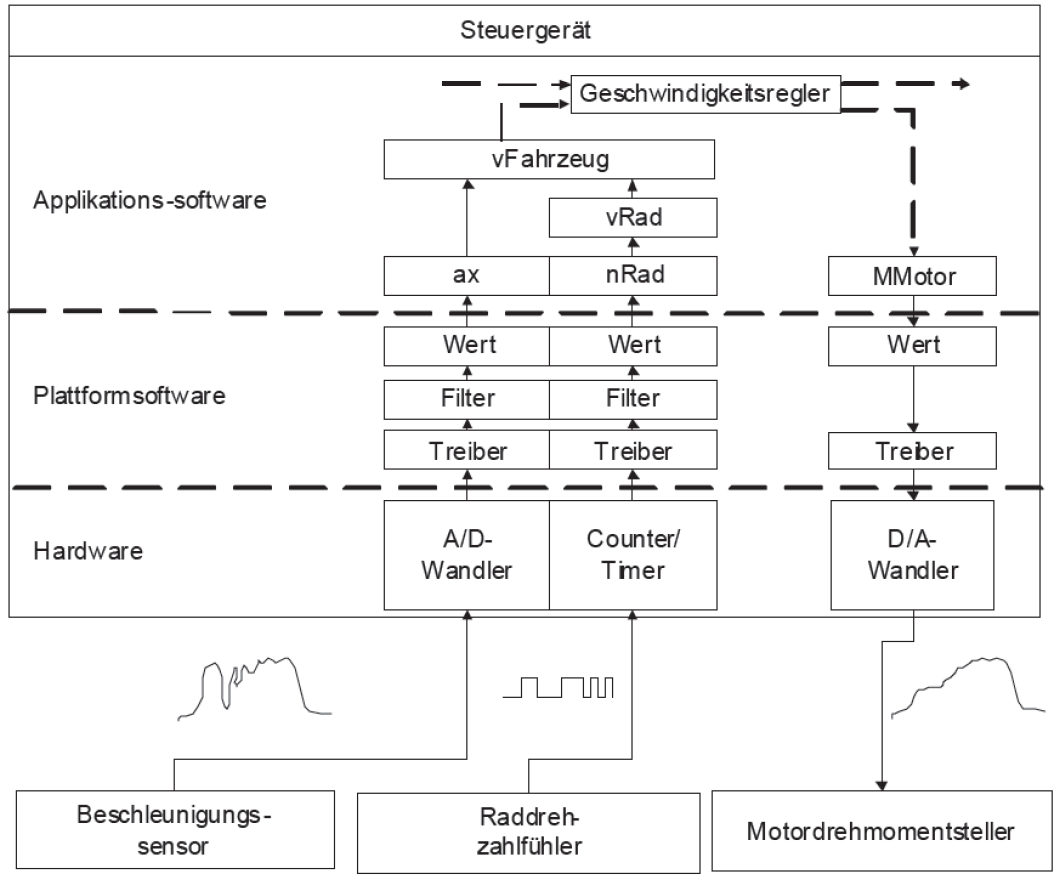
\includegraphics[width=0.8\columnwidth]{images/embedded_system_aufbau_schichten.png}
\end{center}


\subsection{Beispiele}

\vspace{-0.2cm}

\begin{minipage}[t]{0.48\columnwidth}
    \raggedright
    \subsubsection*{Fahrrad-Computer}

    \begin{outline}
        \1 GPS-Navigation
        \1 Geschwindigkeits- und Trittfrequenzmessung
        \1 Pulsmesser
        \1 Drahtlosübertragung (ANT+)
        \1 Interface zu elektronischer Gangschaltung
        \1 Barometer, Thermometer
        \1 Trainingsassistent
        \1 Display
    \end{outline}

    \subsubsection*{Weitere Beispiele}

    \begin{itemize}
        \item Smartphone
        \item Mobile Base Station
        \item CNC-Bearbeitungszentdrum
        % \item Schubumkehr bei Flugzeugen
        % \item Lungenzustandsdetektion mit Elektro-Impedanztomographie (EIT)
        \item Hörgerät
    \end{itemize}
\end{minipage}
\hfill
\begin{minipage}[t]{0.48\columnwidth}
    \raggedright
    \subsubsection*{Auto}

    \begin{outline}
        \1 Sicherheitsrelevante Aufgaben
            \2 ABS, ASR
            \2 Motorenregelung
            \2 Drive-by-wire
            \2 Autonom fahrende Autos
        \1 Unterhaltung / Komfort
            \2 Radio / CD / etc.
            \2 Navigation
            \2 Klima
        \1 Mehrere Netzwerke
            \2 CAN, LIN, Ethernet
        \1 Echtzeitteile und andere
        \1 Von einfachsten $\micro$Cs bis DSPs und GPUs 
    \end{outline}

    \textrightarrow\ Auto ist ein riesiges Embedded System
\end{minipage}


\subsection{Deeply Embedded System}

\begin{itemize}
    \item 'Einfaches' Embedded System, mit \textbf{minimaler Benutzerschnittstelle}, üblicherweise mit \textbf{keinerlei GUI}
        und \textbf{ohne Betriebssystem}
    \item Beschränkt auf \textbf{eine} Aufgabe (z.B. Regelung eines physikalischen Prozesses)
    \item Muss oft zeitliche Bedingungen erfüllen \textrightarrow\ Echtzeitsystem
\end{itemize}


\subsubsection{Beispiele -- Deeply Embedded System}

\begin{minipage}[t]{0.3\columnwidth}
    \begin{itemize}
        \item Hörgerät
        \item Motorenregelung
    \end{itemize}
\end{minipage}
\hfill
\begin{minipage}[t]{0.3\columnwidth}
    \begin{itemize}
        \item ABS-Controller
        \item 'Sensor' im IoT
    \end{itemize}
\end{minipage}
\hfill
\begin{minipage}[t]{0.3\columnwidth}
    \begin{itemize}
        \item etc...
    \end{itemize}
\end{minipage}


\subsection{Betriebssysteme bei Embedded Systems}

\begin{outline}
    \1 Es kommen Betriebssysteme wie (Embedded) Linux oder Android zum Einsatz \\
        \textrightarrow\ \textbf{Achtung: Linux und Android sind nicht echtzeitfähig!}
    \1 Wenn Echtzeit verlangt wird: real-time operating systems (RTOS)
        \2 Beispiele: Zephyr, Free RTOS (Amazon), TI-RTOS (Texas Instuments), etc. \\
            \textrightarrow\ RTOS siehe Abschnitt \ref{Real-Time Operating Systems (RTOS)}
\end{outline}


\subsection{Bare Metal Embedded System}

\begin{itemize}
    \item Es kommt \textbf{keinerlei Betriebssystem} zum Einsatz
    \item Bare Metal Embedded Systems sind recht \textbf{häufig}, insbesondere bei \textbf{Deeply Embedded Systems}
    \item Bare Metal Embedded Systems stellen besondere Ansprüche an Programmierung
\end{itemize}


\subsection{Zuverlässigkeit}

\begin{minipage}[c]{0.45\columnwidth}
    \pgfplotsset{samples=100}   % sample points to make graph smooth

\begin{center}
    \begin{tikzpicture}
        [
            scale = 0.6,
            >=latex
        ]
        \begin{axis}
            [
                title=\textbf{Zuverlässigkeit},
                width=8cm,
                height=5cm,
                xmin=-0.2, xmax=8, ymin=-0.1, ymax=1.3, axis lines=middle,
                x label style={at={(axis description cs:0.5,0)},anchor=north},
                y label style={at={(axis description cs:-0.1,0.5)},rotate=90,anchor=south},
                xlabel=Zeit,
                ylabel=Wahrscheinlichkeit,
                xtick=\empty,
                ytick={0, 0.2, 0.4, 0.6, 0.8, 1, 1.2}
                %grid
            ]
        
            % plot
            \addplot[color=blue, thick, domain=-0:10]{exp(-0.5*x)};
        \end{axis}
        
    \end{tikzpicture}
\end{center}
\end{minipage}
\hfill
\begin{minipage}[c]{0.5\columnwidth}
    \raggedright

    \begin{itemize}
        \item Je länger das System läuft, desto weniger zuverlässig ist es
        \item Die Wahrscheinlichkeit für einen Ausfall steigt stetig
    \end{itemize}
    
    \vspace{0.2cm}

    \textbf{Achtung:} Hier ist nur die Alterung der Hardware berücksichtigt
\end{minipage}


\subsection{Verfügbarkeit}

Die Verfügbarkeit A (availability) ist der Anteil der Betriebsdauer innerhalb dessen das System seine Funktion erfüllt.
$$ \text{Verfügbarkeit} = \frac{\text{Gesamtzeit} - \text{Ausfallzeit}}{\text{Gesamtzeit}} $$


% \subsection{Abstraktionsschichten}

% \begin{itemize}
%     \item Bei $\micro$C-Programmierung (Firmware) müssen oft Bitmuster in Register geschrieben werden
%     \item Solche Register-Zugriffe dürfen \textbf{nicht} 'willkürlich' überall im Code erfolgen \\
%         \textrightarrow\ schlecht lesbar, schlecht portiertbar, fehleranfällig
%     \item \textbf{Damit Code lesbarer und besser auf andere Platform portierbar wird, beinhaltet jeder professionelle Code einen
%         Hardware Abstraction Layer (HAL)}
%     \item HAL führt \textbf{nicht} zum Verlust bei Laufzeit, wenn korrekt implementiert
% \end{itemize}


% \subsubsection{Hardware-abstraction-layer (HAL)}

% \begin{itemize}
%     \item Trennt HW-Implementierung von SW-Logik
%     \item Gleiche SW kann auf verschiedene HW verwendet werden \textrightarrow\ Portabilität
%     \item HW-Komponenten können einfach ausgetauscht werden \textrightarrow\ Flexibilität
% \end{itemize}


        % Modellierung von Embedded (real-time) Systems (Model Driven Development, MDD)
        \section{Real-Time System (Echtzeitsystem)}

\subsection{Definitionen}

\subsubsection{Real-Time System (Echtzeitsystem)}

\begin{itemize}
    \item Ein Echtzeitsystem ist ein System, das Informationen \textbf{innerhalb einer definierten Zeit (deadline) bearbeiten} muss. \\
        \textrightarrow\ Explizite Anforderungen an \textbf{turnaround-time} (Antwortzeit) müssen erfüllt sein
    \item Wenn diese Zeit nicht eingehalten werden kann, ist mit einer \textbf{Fehlfunktion} zu rechnen.
\end{itemize}

\vspace{0.2cm}

\begin{minipage}[t]{0.55\columnwidth}
    \begin{center}
        \myul{\textbf{Typisches Echtzeitsystem}}

        \vspace{0.1cm}

        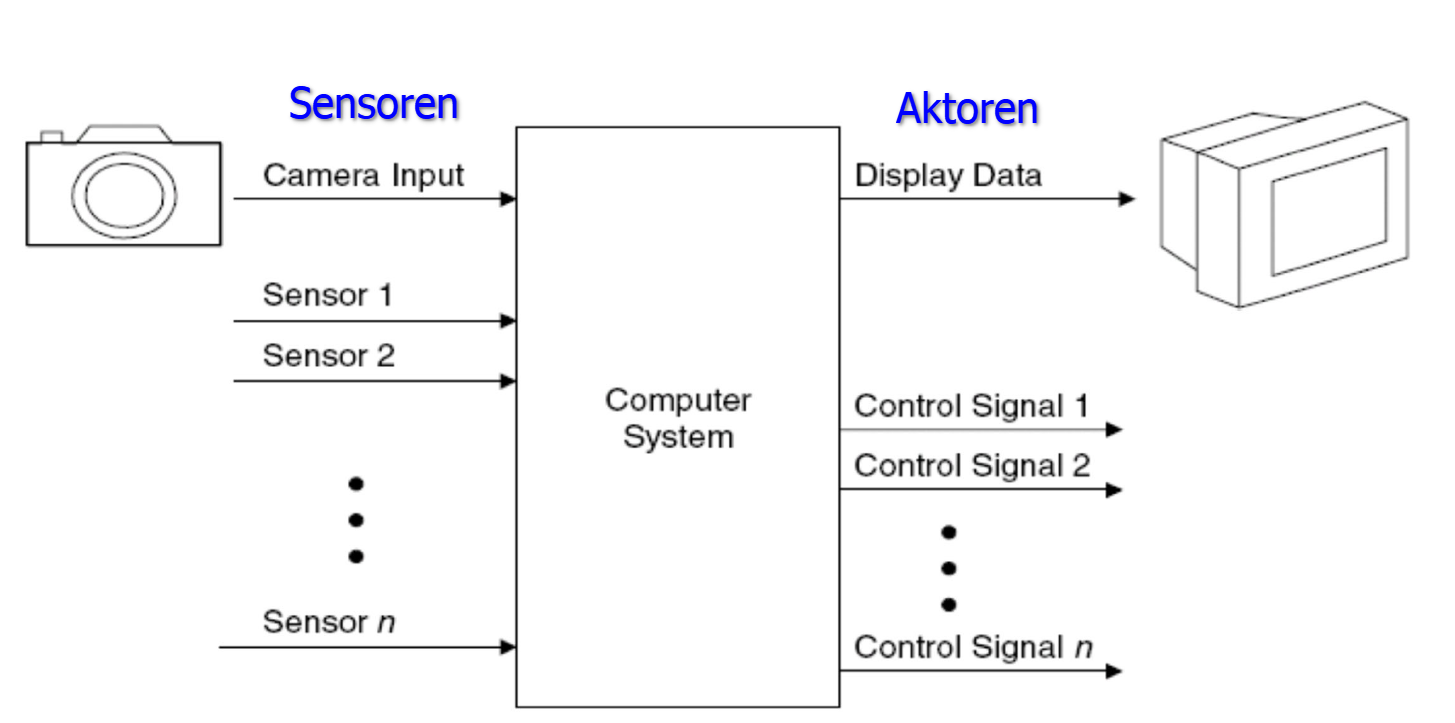
\includegraphics[width=\columnwidth]{images/typisches_echtzeitsystem.png}
    \end{center}
\end{minipage}
\hfill
\begin{minipage}[t]{0.4\columnwidth}
    \begin{center}
        \myul{\textbf{Repräsentation RT-System}}

        \vspace{0.1cm}

        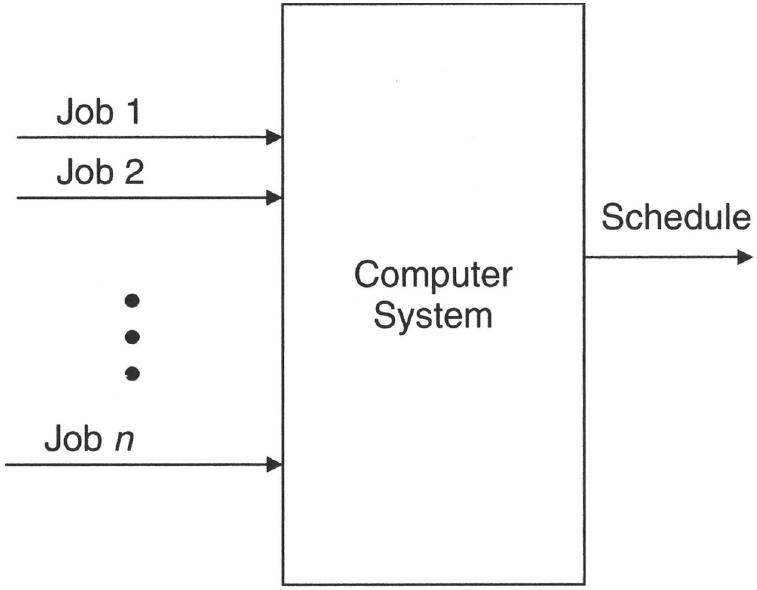
\includegraphics[width=0.7\columnwidth]{images/typische_repraesentation_echtzeitsystem.png}

        Sequenz von Aufgaben (Jobs) müssen zeitlich geplant (scheduled) werden
    \end{center}
\end{minipage}



\subsubsection{Zeitdefinitionen (Task)}

\begin{center}
    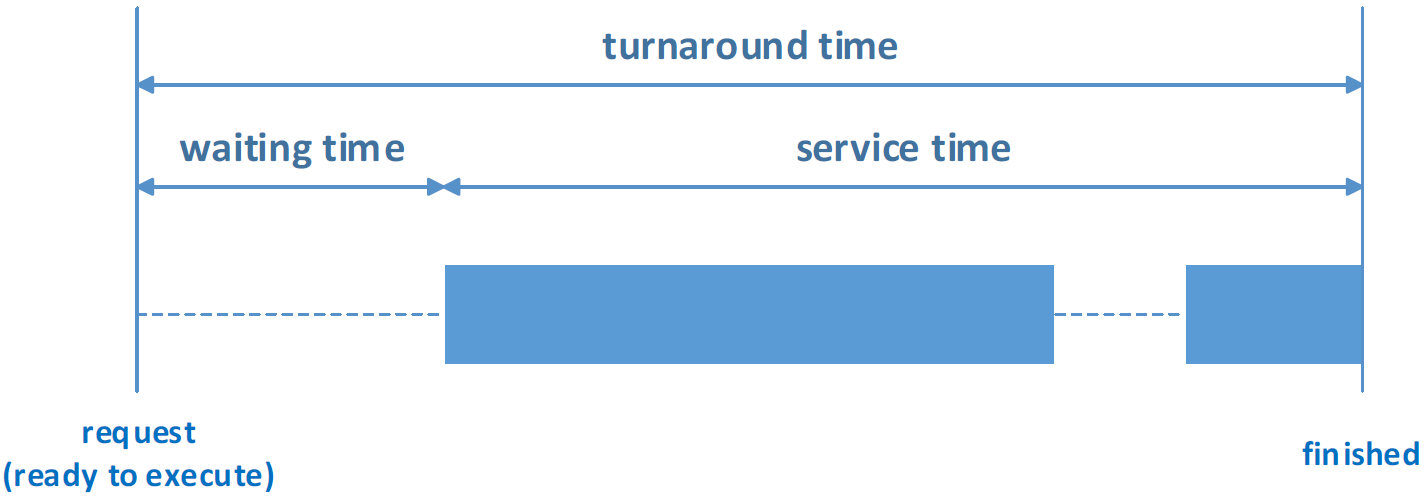
\includegraphics[width=0.7\columnwidth]{images/zeitdefinitionen_task.png}
\end{center}

\begin{outline}
    \1 \textbf{turnaround time:} (response time, Antwortzeit) 
        \2 Startet, wenn der Task bereit zur Ausführung ist und endet, wenn der Task fertig abgearbeitet ist
        \2 Zeit zwischen dem Vorhandensein von Eingangswerten an das System (Stimulus) bis zum Erscheinen der gewünschten Ausgangswerte.
    \1 \textbf{waiting time:} (Wartezeit)
        \2 Zeit zwischen Anliegen der Eingangswert und Beginn der Abarbeitung des Tasks
    \1 \textbf{service time:} (Bearbeitungszeit)
        \2 Zeit für Abarbeitung des Tasks \textrightarrow\ Unterbrechungen bzw. (preemptions) möglich 
\end{outline}


\subsection{Fehlverhalten eines Systems (failed system)}

\begin{itemize}
    \item Ein fehlerhaftes System (failed system = missglücktes System) ist ein System, das nicht alle formal
        definierten Systemspezifikationen erfüllt.
    \item \textbf{Die Korrektheit eines RT Systems bedingt sowohl die Korrektheit der Outputs als auch die Einhaltung
        der zeitlichen Anforderungen.}
\end{itemize}


\subsection{Echtzeitdefinition -- Verschiedene Echtzeitsysteme}

\begin{outline}
    \1 \textbf{soft real-time system} (weiches Echtzeitsystem)
        \2 Durch Verletzung der Antwortzeiten wird das System \textbf{nicht} ernsthaft beeinflusst
        \2 Es kommt zu Komforteinbussen
    \1 \textbf{hard real-time system} (hartes Echtzeitsystem)
        \2 Durch Verletzung der Antwortzeiten wird das \textbf{System ernsthaft beeinflusst}
        \2 Es kann zu einem kompletten Ausfall oder katastrophalem Fehlverhalten kommen
    \1 \textbf{firm real-time system} (festes Echtzeitsystem)
        \2 Kombination aus soft real-time system und hard real-time system
        \2 Durch Verletzung einiger weniger Antwortzeiten wird das System nicht ernsthaft beeinflusst
        \2 Bei vielen Verletzungen der Antwortzeiten kann es zu einem kompletten Ausfall oder katastrophalem Fehlverhalten kommen
\end{outline}


\subsubsection{Beispiele verscheidener Echtzeitsysteme}

\begin{center}
    \begin{tabular}{@{}lll@{}}
        \toprule
        \textbf{System}     & \textbf{Klassifizierung}  & \textbf{Erlärung}                             \\
        \midrule
        Geldautomat         & soft                      & Auch wenn mehrere Deadlines nicht eingehalten \\
                            &                           & werden können, entsteht dadurch keine         \\
                            &                           & Katastrophe. Im schlimmsten Fall erhält ein   \\
                            &                           & Kunde sein Geld nicht.                        \\
        \midrule
        GPS-gesteuerter     & firm                      & Wenn die Positionsbestimmung versagt, könnte  \\
        Rasenmäher          &                           & das Blumenbeet der Nachbarn platt gemäht      \\
                            &                           & werden.                                       \\
        \midrule
        Regelung eines      & hard                      & Das Versagen der Regelung kann dazu führen,   \\
        Quadrocopters       &                           & dass der Quadrocopter ausser Kontrolle        \\
                            &                           & gerät und abstürzt.                           \\
        \bottomrule
    \end{tabular}
\end{center}


% \subsection{Determinsismus (determinacy)}


% \subsection{Auslastung (utilization)}


% \subsection{Real-time Scheduling}

        \section{Modellierung eines Embedded Systems}

\subsection{V-Modell für Software-Entwicklungszyklus}

\begin{center}
    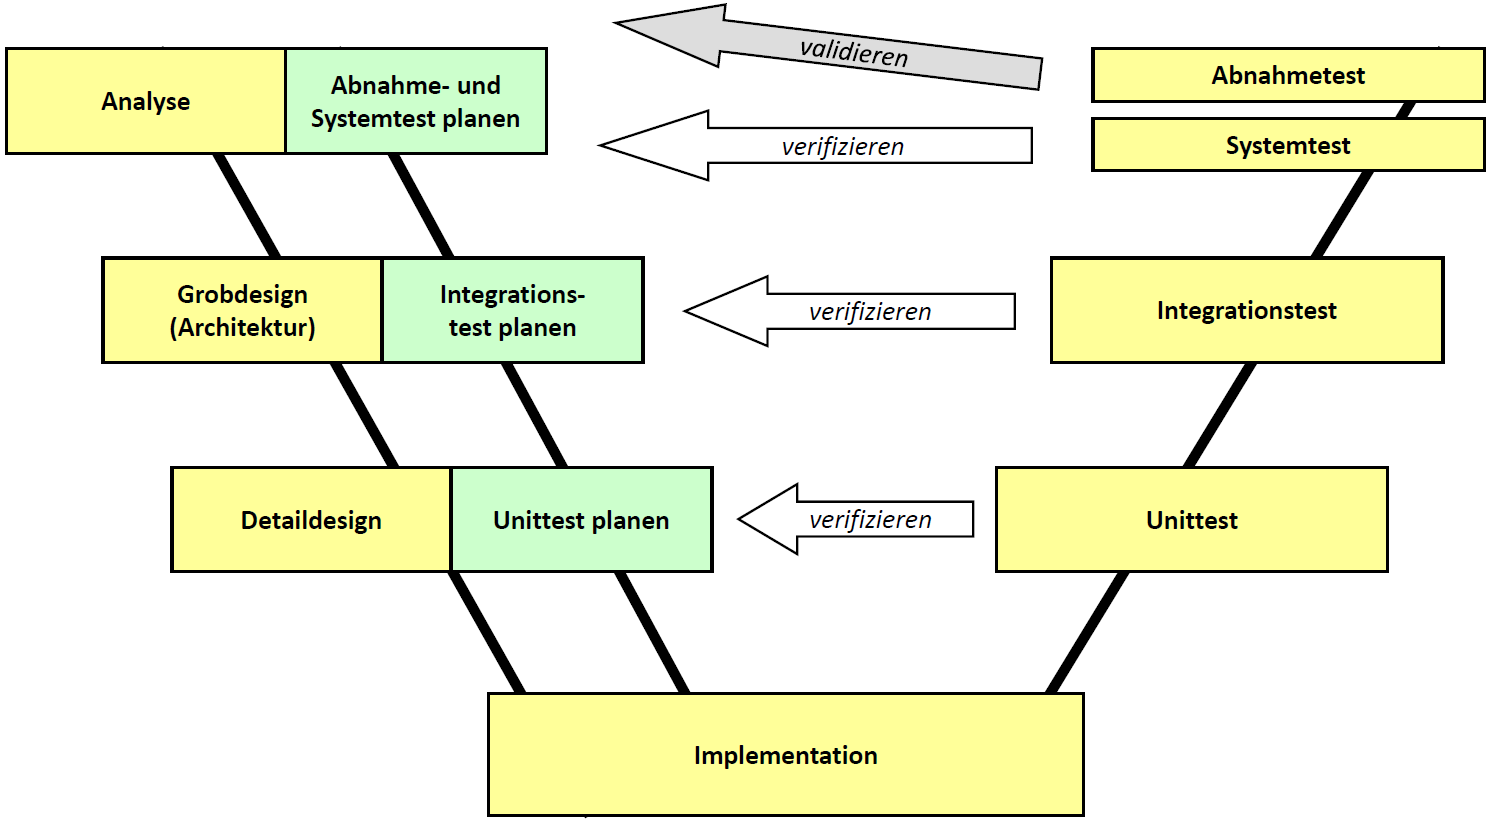
\includegraphics[width=0.7\columnwidth]{images/V_modell.png}
\end{center}

\textrightarrow\ Nur Anforderungen (requirements) definieren, welche man auch testen kann!


\subsection{Model Driven Development (MDD)}

\begin{outline}
    \1 Bei \textbf{modellbasierter Entwicklung} kommen in \textbf{allen Entwicklungsphasen} durchgängig Modelle zum zur Anwendung
    \1 MDD geht davon aus, dass aus formalen Modellen lauffähige Software erzeugt wird \\
        \textrightarrow\ Codegeneratoren
    \1 Modelle werden traditionell als Werkzeug der Dokumentation angesehen
        \2 Unter Umständen wird zweimal dasslbe beschrieben (Code und Diagramm) \\
            \textbf{\textrightarrow\ unbedingt zu vermeiden!}
\end{outline}


\subsection{Vorgehen bei der Modellierung}

\begin{minipage}[c]{0.6\columnwidth}
    \begingroup
    \renewcommand{\outlinei}{enumerate}
    \renewcommand{\outlineii}{itemize}

    \begin{outline}
        \1  \cgn{Systemgrenze definieren}
            \2 Kontextdiagramm: Use-Case-Diagramm
            \2 Kontextdiagramm: Sequenzdiagramm
        \1 \cgn{Systemprozess finden}
            \2 Kontextdiagramm: Use-Case-Diagramm
            \2 Kontextdiagramm: Sequenzdiagramm
        \1 \cgn{Verteilungen festlegen}
            \2 Verteilungsdiagramm (deployment diagram)
        \1 \cbl{Systemprozesse detaillieren}
            \2 Umgangssprachlicher Text
            \2 Sequenzdiagramm
            \2 Aktivitätsdigramm
            \2 Statecharts
            \2 Code (C, C++, ...)
    \end{outline}
    \endgroup
\end{minipage}
\hfill
\begin{minipage}[c]{0.38\columnwidth}
    \raggedright
    \cgn{Stukturmodellierung (Statische Aspekte)}
    
    \vspace{0.2cm}

    \cbl{Modellierung der dynamischen Aspekte}
\end{minipage}


\subsection{Systemgrenze definieren \& Systemprozesse finden}

\subsubsection{Systemgrenze definieren}

\textbf{Die Festlegung der Systemgrenze ist das Wichtigste und Allererste bei sämtlichen Systemen!}

Man sollte sich die folgenden Fragen stellen und diese beantworten:

\vspace{0.1cm}

\begin{outline}
    \1 Was macht das System, d.h. was liegt innerhalb der Systemgrenze?
        \2 Was macht das System  \textbf{nicht}?
    \1 Mit welchen Teilen ausserhalb des Systems kommuniziert das System?
    \1 Welches sind die Schnittstellen zu den Nachbarsystemen (Umsystemen, periheral system)?
\end{outline}


\subsubsection{Systemprozesse finden (use-cases)}

Da man sich noch immer in der \textbf{Analyse} befindet, sollen nur die \textbf{Anforderungen} definiert werden. Die Umsetzung ist Teil
des Designs! \\
Um die Use-Cases zu identifizieren, sollte folgendes beachtet werden:

\vspace{0.1cm}

\begin{outline}
    \1 Aussenbetrachtung des Systems (\textbf{oberflächlich!})
        \2 Nicht komplizierter als nötig
    \1 System als Blackbox betrachten 
        \2 \textbf{Was} soll System können; (nicht: wie soll das System etwas machen)
    \1 RTE-Systeme bestehen häufig aus nur einem einzigen Systemprozess 
        \2 speziell wenn System 'nur' ein Regler ist
\end{outline}


\subsubsection{Kontextdiagramm: Use-Case Diagramm}

\begin{minipage}[t]{0.4\columnwidth}
    \myul{\textbf{Tempomat: zu detailliert}}

    \vspace{0.1cm}

    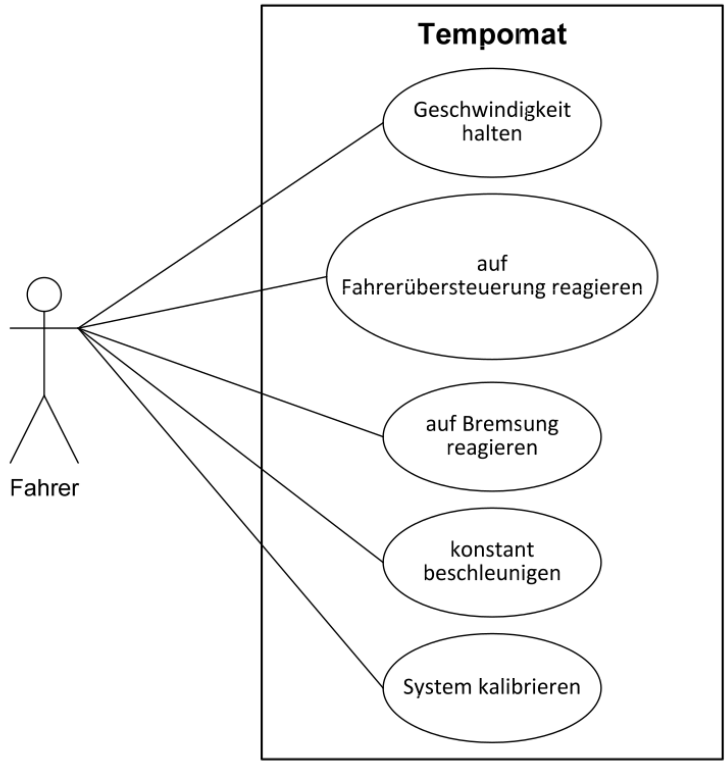
\includegraphics[width=\columnwidth]{images/use-case-diagramm_schlecht.png}
\end{minipage}
\hfill
\begin{minipage}[t]{0.48\columnwidth}
    \myul{\textbf{Tempomat: verbesserte Version}}

    \vspace{0.1cm}

    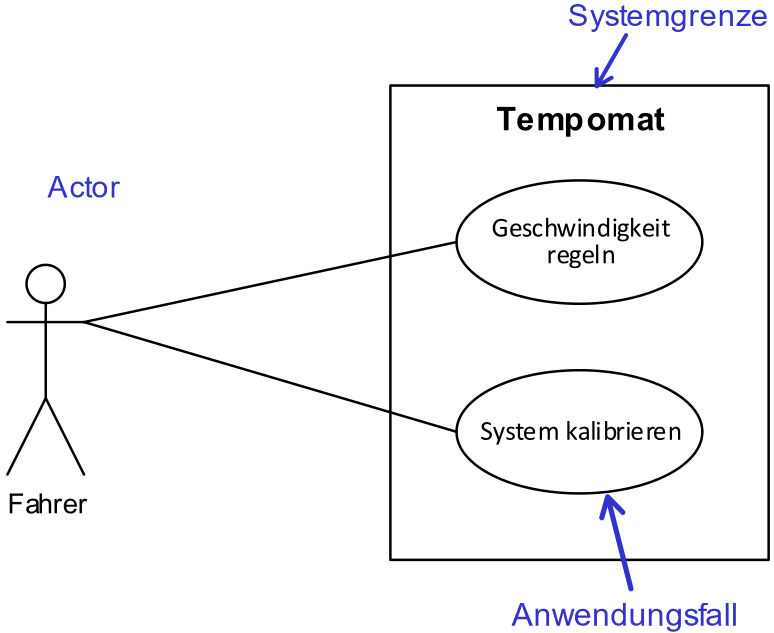
\includegraphics[width=\columnwidth]{images/use-case-diagramm_besser.png}
\end{minipage}


\subsubsection{Kontextdiagramm: Sequenzdiagramm}

\begin{itemize}
    \item Speziell bei Syetemen, deren Grenzen durch \textbf{Nachrichtenflüsse} charakterisiert werden können
    \item Details zu Sequenzdiagrammen siehe Abschnitt % TODO
\end{itemize}


\subsection{Verteilungen festlegen}

\begin{itemize}
    \item Bei Embedded Systems werden häufg \textbf{mehrere Rechnersysteme} verwendet, um die verschiedenen Aufgaben zu erledigen
    \item Rechner sind örtlich verteilt und mittels Kommunikationskanal verbunden \\
        \textbf{\textrightarrow\ Verteilte Systeme (distributed systems)}
\end{itemize}

\vspace{0.2cm}

\begin{minipage}[t]{0.5\columnwidth}
    \raggedright

    \subsubsection{Verteilungsdiagramm}
    
    \begin{description}
        \item[Knoten:] Darstellung der örtlichen Verteilung der Systeme \\
            Knoten können auch hierarchisch aufgebaut sein
        \item[Linien:] Physikalische Verbindungen der Knoten (Netzwerke, Kabel, Wireless, etc.)
    \end{description}
\end{minipage}
\hfill
\begin{minipage}[t]{0.46\columnwidth}
    \example{Tempomat}
    
    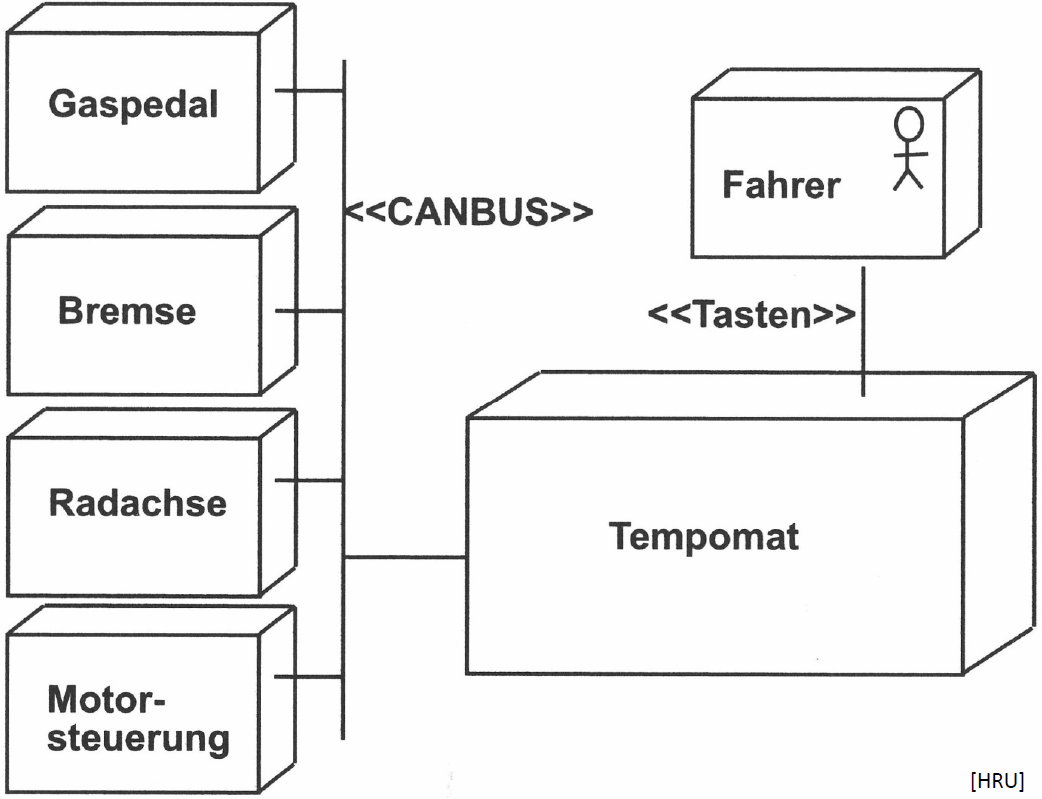
\includegraphics[width=\columnwidth]{images/verteilungsdiagramm_tempomat.png}
\end{minipage}


\subsection{Systemprozesse detaillieren}

\begin{outline}
    \1 Die gefundenen Systemprozesse (use-cases) müssen genauer spezifiziert werden
        \2 \textbf{Nicht detaillierter spezifizieren als sinnvoll / gefordert!}
        \2 Jede weitere Spezifizierung soll eien 'added value' liefern
    \1 Verschiedene Detaillierungsstufen für verschiedene Zielgruppen
        \2 Auftraggeber: Überblick (z.B. in Form von Umgangssprachlichem Text)
        \2 Systementwickler: 'Normale Sicht' enthält mehr Details
\end{outline}


\subsubsection{Sequenzdiagramm}


        % Hardware/Software Codesign
        \section{Hardware-Software-Codesign}

\subsection{Ziele}

\begin{itemize}
    \item Entwurf (Design) \textbf{so lange wie sinnvoll} (nicht so lange wie möglich) \textbf{lösungsneutral}
    \item \textbf{Systemdesign fördern}, statt separate Designs für Mechanik, Elektronik, Firmware, Software, etc., die sich
        unter Umständen auch widersprechen können
    \item Systemspezifikation erfolgt idealerweise mit Hilfe einer \textbf{eindeutigen Spezifikationssprache}, nicht in
        Prosa
    \item Die Spezifikation sollte simuliert (ausgeführt) werden können
    \item Implementationen können einfach geändert werden: HW \textlrarrow\ SW
    \item Zielplattformen: diskrete Elektronik, ASIC, \textmu C, DSP, \textbf{FPGA}, Software
\end{itemize}


\subsection{Anforderungen für praktische Anwendungen}

\begin{outline}
    \1 Methoden / Tools sollten beim Systemdesign nicht zu fachlastig sein
        \2 Methoden sollten für Elektronik-, Firmware- und wenn möglich auch Mechanikentwickler anwendbar sein
    \1 Wenn möglich gute Toolunterstützung
    \1 (Automatische Synthese aus dem Modell)
\end{outline}


\subsection{Spezifikationssprachen}

\begin{minipage}[t]{0.48\columnwidth}
    \raggedright
    \begin{itemize}
    \item \textbf{Formale Sprachen sind eindeutig} \\
        (Prosa immer mehrdeutig)
    \item Spezifikation kann compiliert und ausgeführt werden \textrightarrow\ Simulationen
    \item Die ausführbare Spezifikation dient als \textbf{Golden Reference} für die künftigen Entwicklungsschritte
\end{itemize}
\end{minipage}
\hfill
\begin{minipage}[t]{0.48\columnwidth}
    \myul{\textbf{Beispiele für Spezifikationssprachen}}

    \vspace{0.1cm}

    \begin{itemize}
        \item SystemC (eine C++-Template Library)
        \item SysML
        \item SpecC
        \item SystemVerilog
        \item Esterel
        \item Matlab/Simulink
        \item Statecharts
    \end{itemize}
\end{minipage}


\subsection{Virtuelle Prototypen}

\begin{itemize}
    \item Die Simulation des Systems kann unterschiedlich stark detailliert werden
    \item \textbf{Die simulierten Systeme sind Virtuelle Prototypen}
    \item Während der Entwicklung können einzelne (virtuelle) Teile des Prototyps laufend durch physische Teile
        ersetzt werden
\end{itemize}


\subsection{X-in-the-loop}

\begin{outline}
    \1 \textbf{Model-in-the-Loop (MIL):} Vollständig als Modell vorliegender virtuellen Prototyp
    \1 Je mehr der Prototyp durch konkretere Implementationen ersetzt wird, spricht man von
        \2 Software-in-the loop (SIL)
        \2 Processor-in-the loop (PIL)
        \2 Hardware-in-the loop (HIL)
\end{outline}

\vspace{0.2cm}

\textrightarrow\ Test outputs werden jeweils mit \textbf{Golden Reference} verglichen
\begin{center}
    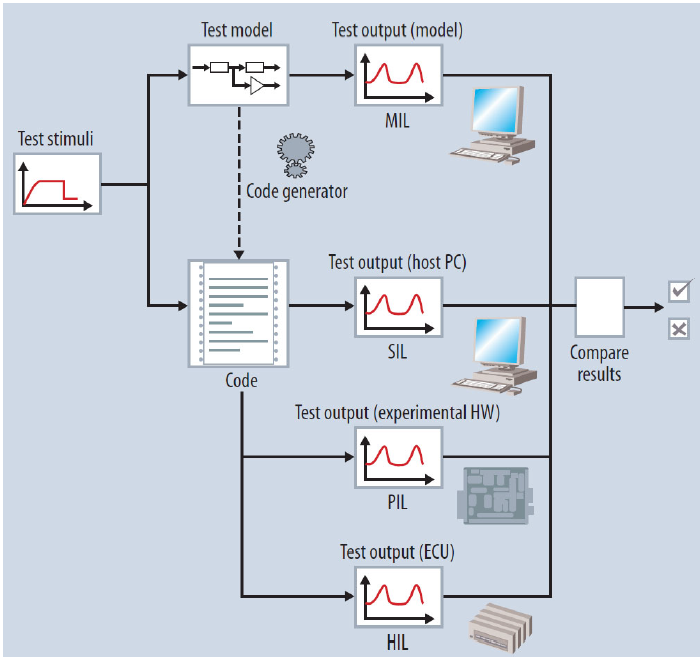
\includegraphics[width=0.9\columnwidth]{images/x_in_loop_testing.png}
\end{center}


\subsection{Entwicklungsplattformen}

Als Entwicklungsplattformen eignen sich häufig \textbf{FPGA basierte Systeme.}

\begin{outline}
    \1 Hardware mit VHDL
    \1 Software/Firmware in C/C++
        \2 auf integriertem \textmu C (z.B. Zynq von AMD/Xilinx) (Hard Core)
        \2 auf Soft Core innerhalb FPGA (z.B. Nios II von Intel/Altera)
\end{outline}


        % Finite State Machines (Anwendung, Implementationen in C und C++)
        \section{Zustandsbasierte Systeme}

\subsection{Asynchrone vs. synchrone FSM}

\begin{minipage}[t]{0.48\columnwidth}
    \raggedright
    \begin{outline}
        \1 \textbf{Asynchron}
            \2 geänderte Inputsignale führen \textbf{direkt} zur Zustandsänderung
            \2 schneller, aber enorm anfällig auf Glitches
    \end{outline}
\end{minipage}
\hfill
\begin{minipage}[t]{0.48\columnwidth}
    \raggedright
    \begin{outline}
        \1 \textbf{Synchron}
            \2 Inputsignale werden nur zu diskreten Zeitpunkten betrachtet \\
                \textrightarrow\ getaktete Systeme
    \end{outline}
\end{minipage}

\vspace{0.2cm}
%TODO: check if this is finished
\begin{outline}
    \1 Softwareimplementationen sind eigentlich immer \textbf{synchron}, da Rechner getaktet sind
    \1 Rein softwareseitig besteht die Problematik der Asynchronizität nicht
\end{outline}


\subsection{Finite State Machines (FSM)}


\subsubsection{Mealy-Automat}

\subsubsection{Moore-Automat}
% Bondi: alles als Moore modellieren

\subsubsection{Medvedjev}
%hier nicht weiter behandelt...?
% Zustand = Output


\subsection{State-Event-Diagramm (Zustandsdiagramm)}

% Beschreibung


\example{State-Event-Diagramm -- Moore Automat}

% \begin{center}
%     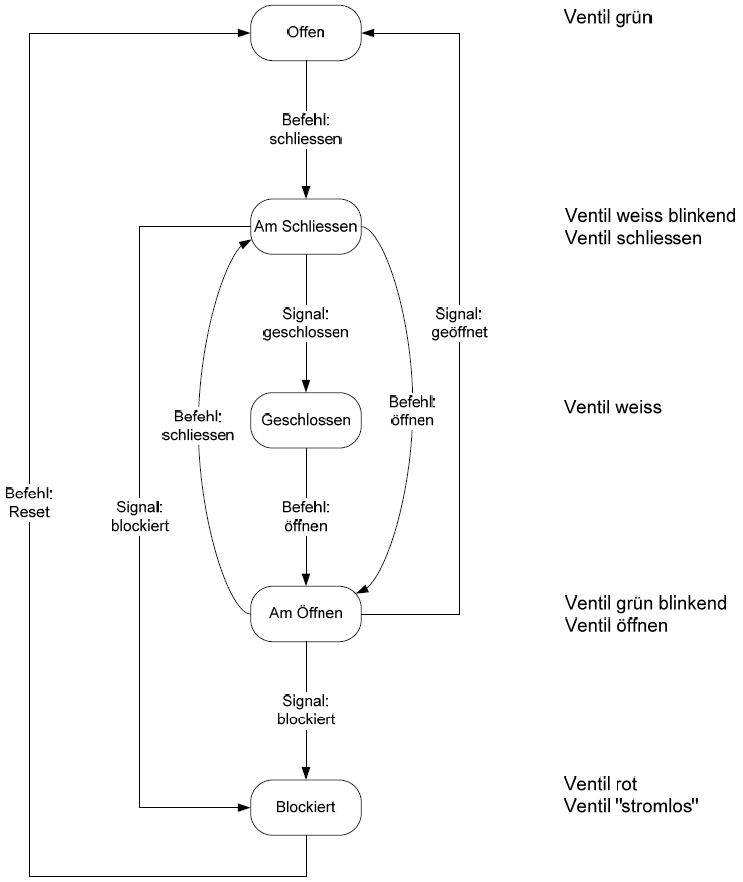
\includegraphics[width=0.8\columnwidth]{images/state_event_example.png}
% \end{center}


        \section{Statecharts}

\subsection{Nachteile von State-Event-Diagrammen}

\begin{itemize}
    \item Zustandsdiagramme sind flach (es gibt keine Hierarchie) \textrightarrow\ schnell unübersichtlicht
    \item Es kann keine zeitliche Parallelität modelliert werden
\end{itemize}


\subsection{Definitionen}


\subsubsection{Elemehte der Statecharts}



\subsection{Hierarchie}


\subsection{Default-State}


\subsection{History}

\subsubsection{Shallow History}


\subsubsection{Deep History}



\subsection{Parallelität}


\subsection{Timers}



\subsection{Beispiel -- Armbanduhr als Statechart}  %CHECK: vielleicht gibt es im Praktikum ein besseres Beispiel...?


        \section{Realisierung flache FSM}

\subsection{Mögliche Realisierungen von flachen FSMs}

\begin{outline}
    \1 Steuerkonstrukt (typischerweise mit \textbf{switch-case})
        \2 prozedural oder objektorientiert
    \1 Definition und Abarbeitung einer \textbf{Tabelle}
        \2 prozedural oder objektorientiert
    \1 \textbf{State Pattern} (Gang of Four, GoF)
        \2 nur objektorientiert
    \1 Generisch mit Templates
        \2 nur mit einer Sprache, die Templates unterstützt (z.B. C++)
\end{outline}

\vspace{0.2cm}

\textrightarrow\ Alle Varianten haben wie immer sowohl Vor- als auch Nachteile \\
\textrightarrow\ Bei allen Varianten sind auch Variationen vorhanden


\subsection{Realisieurng mit Steuerkonstrukt (prozedural in C)}

\subsubsection{State-Event-Diagram -- Up/Down-Counter}

\begin{center}
    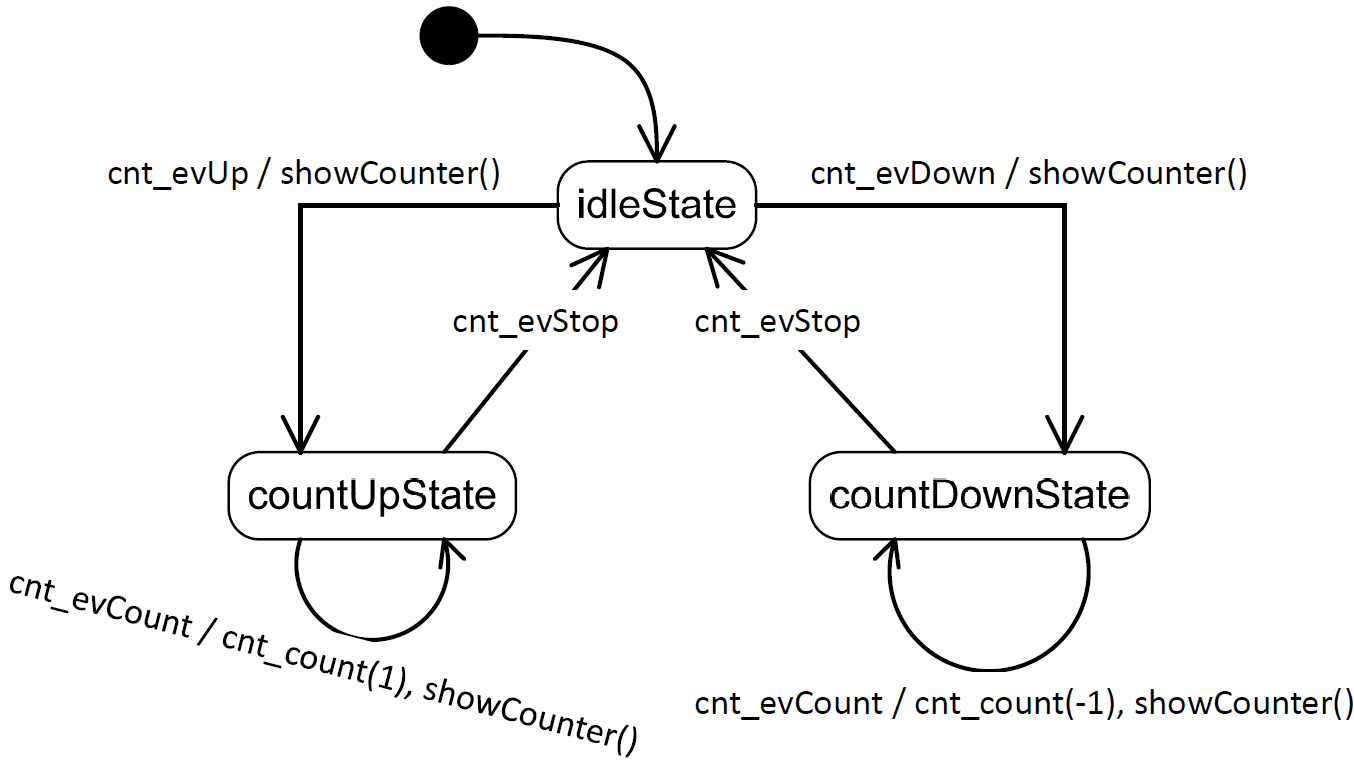
\includegraphics[width=0.7\columnwidth]{images/fsm_up-down-counter_diagramm_C.png}
\end{center}


\subsubsection{Implementation der Prozeduralen Realisierung in C}

\begin{outline}
    \1 \textbf{Ereignisse (events)}
        \2 Schnittstelle nach aussen \textrightarrow\ ändern Zustand der FSM
        \2 In enum definiert (\textbf{public}) \textrightarrow\ header-file
        \2 Einzelne Events und enum Bezeichnung enthalten \textbf{Unitkürzel} (hier: \mylstbox{cnt_})
    \1 \textbf{Zustände (states)}
        \2 In enum definiert (\textbf{nicht} public) \textrightarrow\ sourcecode-file
    \1 \textbf{Aktueller Zustand} wird in einer \textbf{statischen Varianlen} gehalten
    \1 Die FSM wird in \textbf{zwei Funktionen} implementiert
        \2 Initialiserungs-Funktion (hier: \mylstbox{void cnt_ctrlInit(int initValue)})
        \2 Prozess-Funktion (hier: \mylstbox{void cnt_ctrlProcess(cnt_Event e)}) \\
            \textrightarrow\ Zustände prüfen, Zustandsübergänge veranlassen
    \1 Anstossen einer FSM
        \2 Initialisierung in \lstinline|main|-Funktion
        \2 Überprüfung, welches Event aufgetreten ist meist in \mylstbox{do-while}-Schleife
\end{outline}


\subsubsection{Eigenschaften der Prozeduralen Realisierung in C}

\begin{outline}
    \1 Da aktueller Zustand eine statische Variable ist, kann es nur \textbf{eine einzige Instanz} der FSM geben
    \1 Bei mehreren Instanzen in C...
        \2 darf \mylstbox{currentState} nicht \mylstbox{static} sein und muss als Parameter mitgegenen werden,
            bzw. ein Pointer auf die jeweilige Variable
        \2 Zustands-enum muss in die Schnittstelle (header-file) oder es muss z.B. mit \mylstbox{void*} gearbeitet werden
    \1 In C ist \textbf{keine schöne Kapselung} der Attribute möglich (\mylstbox{currentState})
    \1 Funktion \mylstbox{cnt_ctrlProcess()} kann beliebig aufgerufen werden (periodischer Task, laufend, etc.)
    \1 Bei exponierten Funktionen / Definitionen muss in C ein Unitkürzel vorangestellt werden (hier: \mylstbox{cnt_})
\end{outline}


\example{Up/Down-Counter (prozedural in C)}

% TODO: \para environment not showing...?
% TODO: add keywords and stuff to listings setup

\begin{minipage}[t]{0.48\columnwidth}
    \para{Schnittstelle Counter in C} 
    \lstinputlisting{snippets/fsm_procedural_C/fsm_counter_C.h}
\end{minipage}
\hfill
\begin{minipage}[t]{0.48\columnwidth}
    \para{Implementation Counter in C} 
    \lstinputlisting{snippets/fsm_procedural_C/fsm_counter_C.c}
\end{minipage}


\para{Schnittstelle FSM in C} 
\lstinputlisting{snippets/fsm_procedural_C/fsm_counterCtrl_C.h} 

\para{Implementation FSM in C} 
\lstinputlisting{snippets/fsm_procedural_C/fsm_counterCtrl_C.c}

\para{Anstossen der FSM in C} 
\lstinputlisting{snippets/fsm_procedural_C/fsm_main_counterTest_C.c}



\subsection{Realisieurng mit Steuerkonstrukt (objektorientiert in C++)}
\label{Realisieurng mit Steuerkonstrukt (objektorientiert in CPP)}

\subsubsection{State-Event-Diagram -- Up/Down-Counter}
\label{State-Event-Diagram -- Up/Down-Counter in CPP}

\begin{center}
    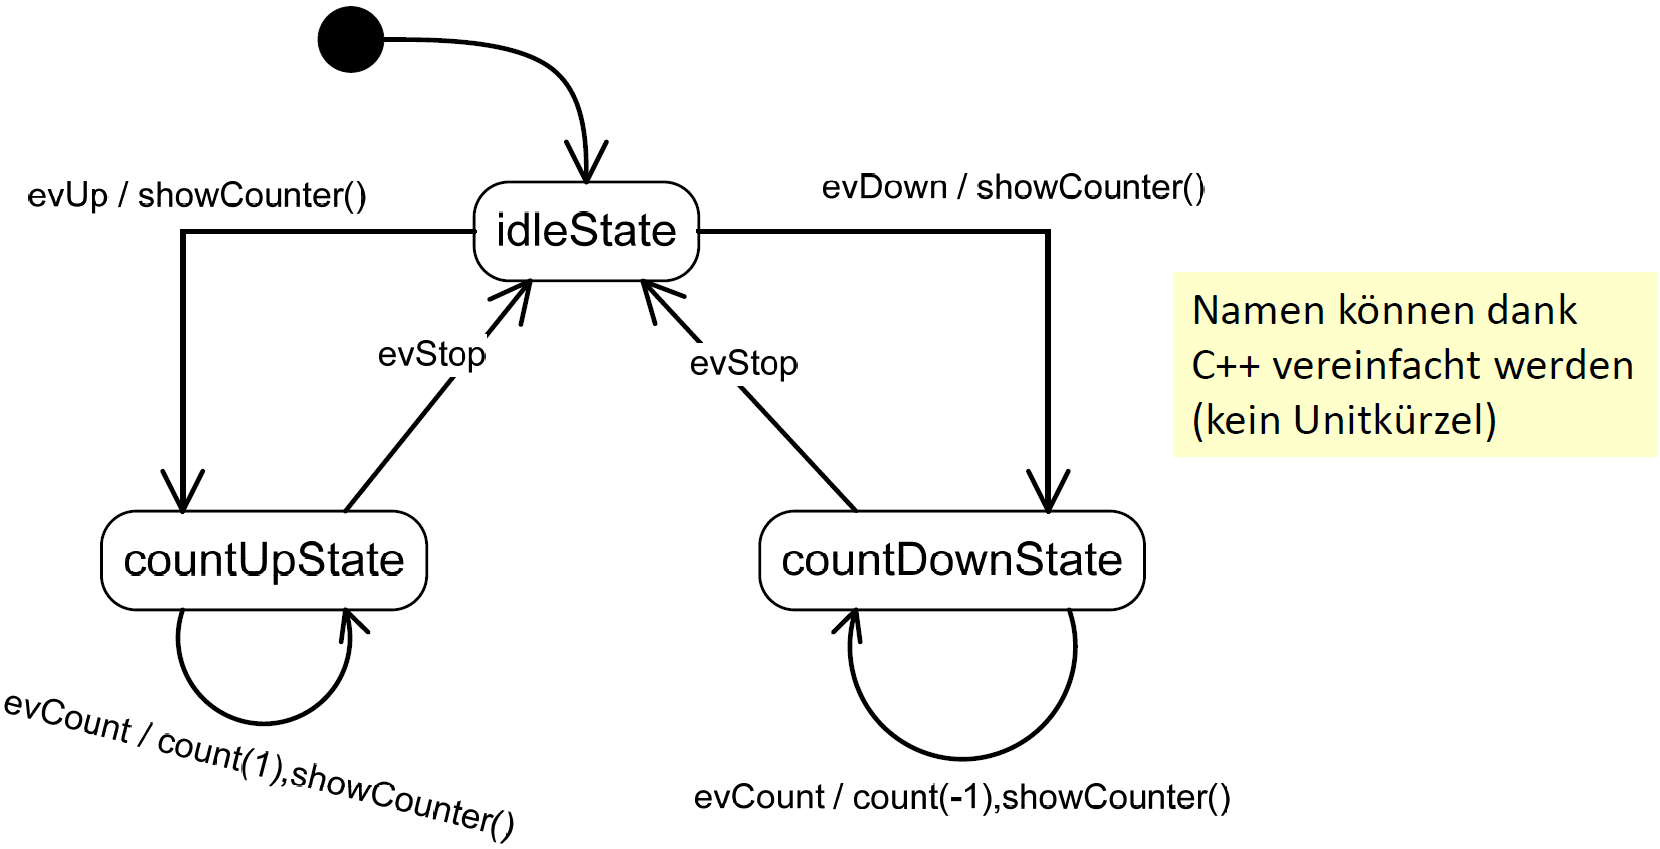
\includegraphics[width=0.7\columnwidth]{images/fsm_up-down-counter_diagramm_CPP.png}
\end{center}


\subsubsection{Zusammenhang der Klassen Counter und CounterCtrl}
\label{Zusammenhang der Klassen Counter und CounterCtrl}

\begin{center}
    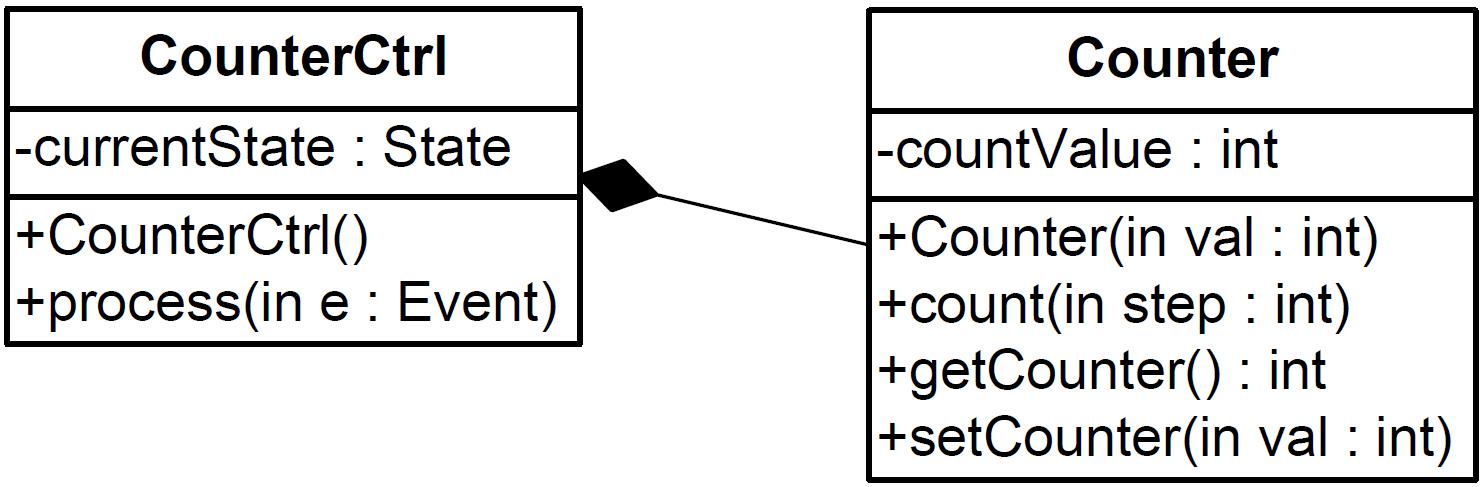
\includegraphics[width=0.7\columnwidth]{images/fsm_CPP_klassendiagramm.png}
\end{center}

\begin{outline}
    \1 Klasse \mylstbox{Counter} führt eigentliche Rechenaufgaben durch
        \2 ist bei \textbf{allen} (objektorientierten) Realiseurngsarten \textbf{identisch}
    \1 Klasse \mylstbox{CounterCtrl} ist FSM, welche Zugriff auf den Counter steuert 
\end{outline}

\textbf{ \textrightarrow\ Generell sollten Steuerung und Element, das gesteuert wird, getrennt werden!}


\subsubsection{Implementation der Prozeduralen Realisierung in C++}

\begin{outline}
    \1 \textbf{Ereignisse (events)}
        \2 Schnittstelle nach aussen \textrightarrow\ ändern Zustand der FSM
        \2 Im \textbf{public} Teil der Klasse als enum definiert
        \2 Keine Unitkürzel nötig
    \1 \textbf{Zustände (states)}
        \2 Im \textbf{private} Teil der Klasse als enum definiert \textrightarrow\ header-file
    \1 \textbf{Aktueller Zustand} \mylstbox{currentState} wird in \textbf{privatem Attribut} von \mylstbox{CounterCtrl} gehalten
    \1 Die FSM wird in \textbf{zwei Funktionen} implementiert
        \2 Kontruktor (hier: \mylstbox{CounterCtrl::CounterCtrl(int initValue=0)})
        \2 Prozess-Funktion (hier: \mylstbox{void CounterCtrl::process(CounterCtrl::Event e)}) \\
            \textrightarrow\ Zustände prüfen, Zustandsübergänge veranlassen
    \1 Anstossen einer FSM
        \2 Initialisierung in \lstinline|main|-Funktion
        \2 Überprüfung, welches Event aufgetreten ist meist in \mylstbox{do-while}-Schleife
\end{outline}


\example{Up/Down-Counter (prozedural in C++)}

% TODO: \para environment not showing...?
% TODO: add keywords and stuff to listings setup

\begin{minipage}[t]{0.44\columnwidth}
    \para{Schnitstelle Counter in C++} 
    \lstinputlisting{snippets/fsm_procedural_CPP/fsm_Counter_CPP.h}
\end{minipage}
\hfill
\begin{minipage}[t]{0.52\columnwidth}
    \para{Implementation Counter in C++} 
    \lstinputlisting{snippets/fsm_procedural_CPP/fsm_Counter_CPP.cpp}
\end{minipage}


\para{Schnittstelle FSM in C++} 
\lstinputlisting{snippets/fsm_procedural_CPP/fsm_CounterCtrl_CPP.h} 

\para{Implementation FSM in C++} 
\lstinputlisting{snippets/fsm_procedural_CPP/fsm_CounterCtrl_CPP.cpp}

\para{Anstossen der FSM} 
\lstinputlisting{snippets/fsm_procedural_CPP/fsm_main_counterTest_CPP.cpp}



\subsection{Realisierung mit Tabelle}

\subsubsection{State-Event-Diagram -- Up/Down-Counter}

Siehe Abschnitt \ref{State-Event-Diagram -- Up/Down-Counter in CPP}


\subsubsection{FSM in Tabellenform}

Das State-Event-Diagramm wird in eine Tabelle 'übersetzt'. \textbf{Jede Zeile der Tabelle entspricht einer Transition (Pfeil) im 
State-Event-Diagramm}

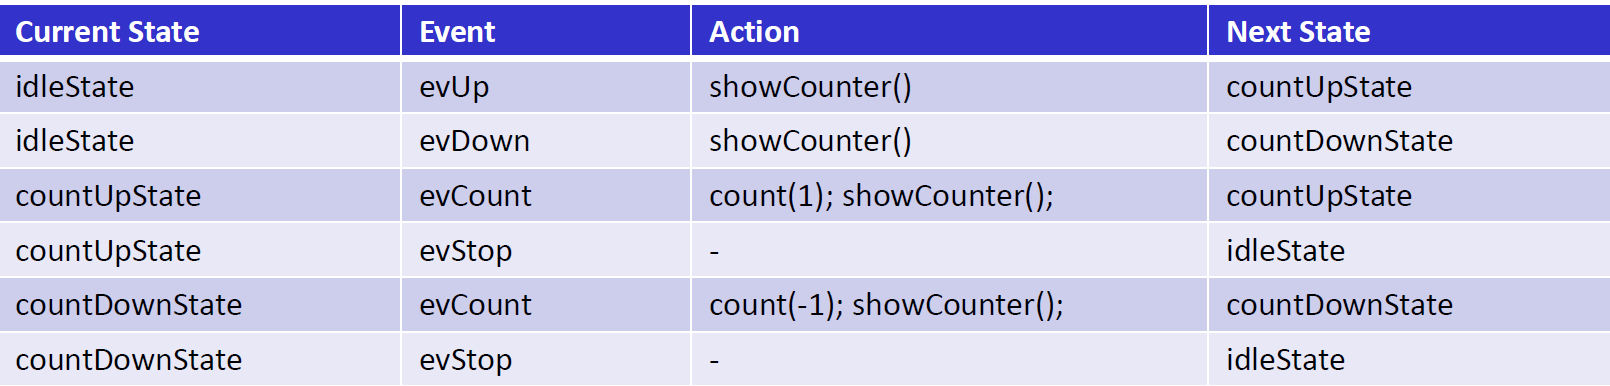
\includegraphics[width=\columnwidth]{images/fsm_tabelle.png}


\subsubsection{Implementation der Realisierung mittels Tabelle in C++}

\begin{outline}
    \1 Die ganze FSM ist in einer Tabelle gespeichert
    \1 \textbf{Aktionen} sind als \textbf{Funktion} implementiert, in der \textbf{Tabelle} steht der entsprichende \textbf{Funktionspointer} % CHECK: sind das Pointer auf Klassenelemente?
    \1 \textbf{Abarbeitung} der FSM erfolgt mittels \textbf{Execution Engine}, die in der Tabelle 'nachschaut', was zu tun ist
        \2 Execution Engine \textbf{ändert sich nicht}, wenn FSM geändert wird!
    \1 \textbf{Transition} wird als klasseninterner \mylstbox{struct} deklariert
        \2 enthält aktuellen Zustand, Event, Funktionspointer auf Aktionsmethode und nächsten Zustand
    \1 \textbf{FSM} wird als statischer, offener Array deklariert
        \2 Hier wird ganze FSM gespeichert
        \2 ein \mylstbox{struct} bildet konkret eine Zeile der Tabelle ab
\end{outline}


\subsubsection{Eigenschaften der Realisierung mittels Tabelle}

\begin{outline}
    \1 Die Tabelle kann prozedural oder \textbf{objektorientiert} implementiert werden
        \2 Objektorientierte Variante verwendet einzig die Datenkapselung (keine Vererbung, kein Polymorphismus)
        \2 Objektorientierte Variante ist klarer / schöner strukturiert
    \1 \textbf{Aktions-Funktionen} können \textbf{nicht inlined} werden, da ein Pointer auf die Funktionen verwendet wird
\end{outline}


\subsubsection{Tabelle vs. prozedural}

\begin{minipage}[t]{0.48\columnwidth}
    \raggedright
    \myul{\textbf{Gemeinsamkeiten}}
    
    \vspace{0.1cm}

    \begin{outline}
        \1 Testprogramm \mylstbox{counterTest.cpp}
        \1 Schnittstelle (public-Teil) von Klasse \mylstbox{CounterCtrl}
        \1 Gesamte Klasse \mylstbox{Counter}
    \end{outline}
\end{minipage}
\hfill
\begin{minipage}[t]{0.48\columnwidth}
    \raggedright
    \myul{\textbf{Unterschiede}}
    
    \vspace{0.1cm}

    \begin{outline}
        \1 private-Teil von Klasse \mylstbox{CounterCtrl} und Implementation davon
    \end{outline}
\end{minipage}


\example{Up/Down-Counter (mit Tabelle in C++)}

\para{Schnittstelle FSM in C++} 
\lstinputlisting{snippets/fsm_table_CPP/fsm_CounterCtrl_table_CPP.h} 

\para{Implementation FSM in C++} 
\lstinputlisting{snippets/fsm_table_CPP/fsm_CounterCtrl_table_CPP.cpp}


\subsection{Erweiterung der Realisierung mittels Tabellen}

\begin{itemize}
    \item Wenn der Zustandsübergang nicht durch einen Event, sondern eine \textbf{komplexere Prüfung (Event und Guard)} ausgelöst wird, 
        dann könnte der \textbf{Event-Eintrag} in der Tabelle durch einen weiteren \textbf{Funktionspointer} auf eine 
        \textbf{Checkfunktion ersetzt} werden.
    \item Ergänzung für die Behandlung von Entry- und Exit-Actions
\end{itemize}


\example{Up/Down-Counter (mit Checker-Tabelle in C++)}

\begin{outline}
    \1 Änderungen in \mylstbox{CounterCtrl.h} \textrightarrow\ siehe Beispiel-Code
    \1 Änderungen in \mylstbox{CounterCtrl.cpp}
        \2 checker-Funktionen müssen implementiert werden
        \2 In Tabelle steht statt Event die Adresse der checker-Funktion (analog zu action-Funktionen)
\end{outline}

\lstinputlisting{snippets/fsm_table_CPP/fsm_CounterCtrl_table_pChecker_CPP.h}



\subsection{Realisieurng mit StatePattern (ohne actions)}

\subsubsection{Grundidee von StatePatterns}
\label{Grundidee StatePatterns}

\begin{center}
    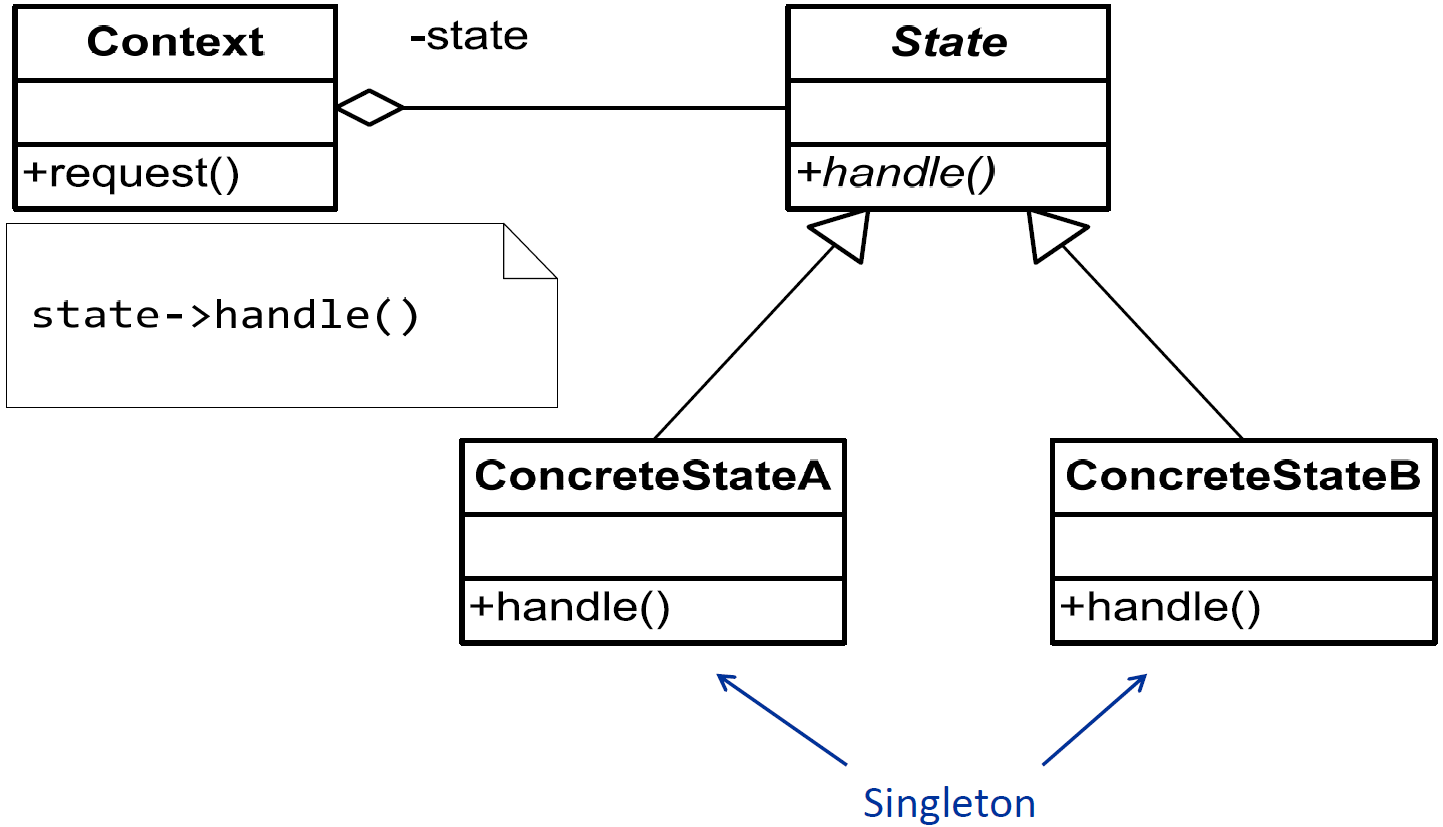
\includegraphics[width=0.7\columnwidth]{images/fsm_state_pattern_struktur.png}
\end{center}

%TODO: slides 4 + 6



\subsubsection{State-Event-Diagram -- Up/Down-Counter}
\label{State-Event-Diagram -- Up/Down-Counter - StatePattern}

\begin{center}
    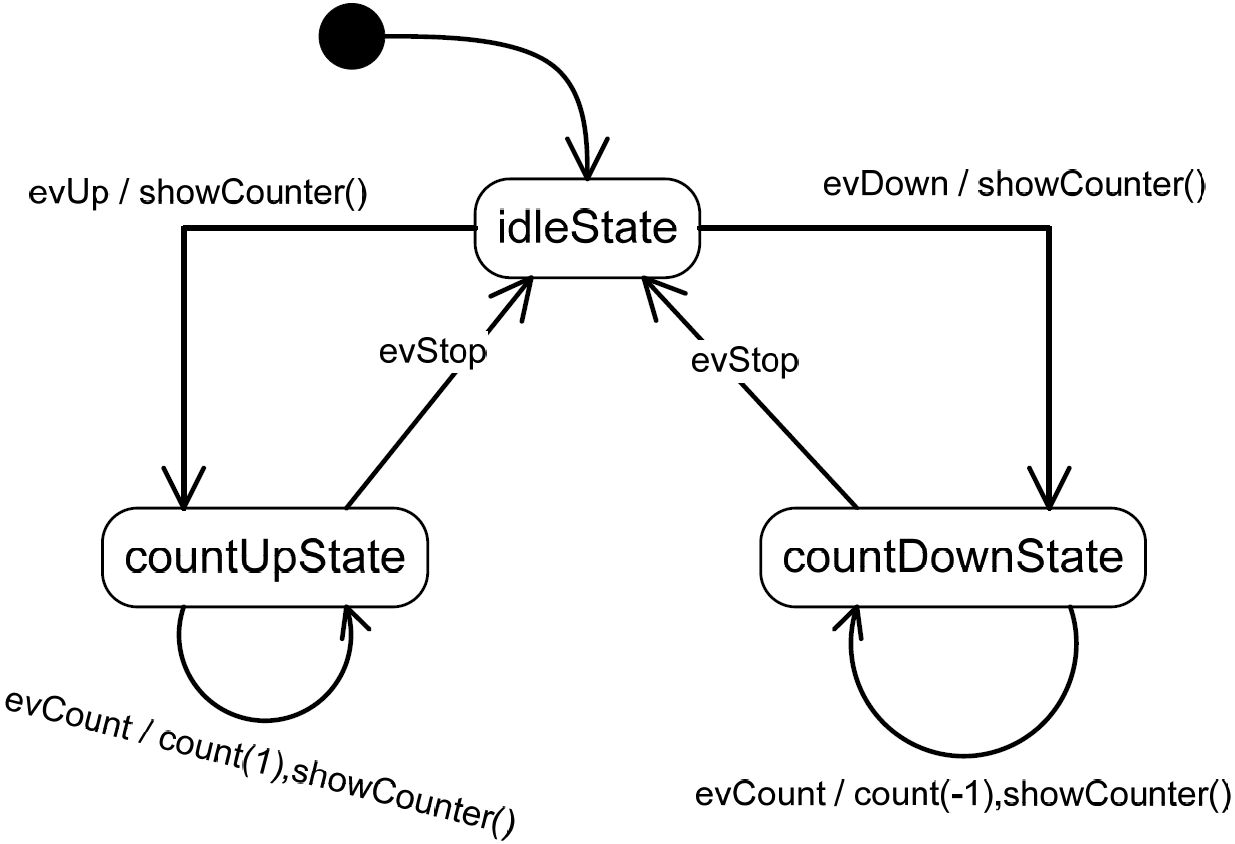
\includegraphics[width=0.7\columnwidth]{images/fsm_up-down-counter_diagramm_state_pattern.png}
\end{center}



\subsubsection{Implementation der Realisierung mittels StatePattern}

%TODO: describe stuff with StatePattern...
% \begin{outline}
%     \1 \textbf{Ereignisse (events)}
%         \2 Schnittstelle nach aussen \textrightarrow\ ändern Zustand der FSM
%         \2 Im \textbf{public} Teil der Klasse als enum definiert
%         \2 Keine Unitkürzel nötig
%     \1 \textbf{Zustände (states)}
%         \2 Im \textbf{private} Teil der Klasse als enum definiert \textrightarrow\ header-file
%     \1 \textbf{Aktueller Zustand} \mylstbox{currentState} wird in \textbf{privatem Attribut} von \mylstbox{CounterCtrl} gehalten
%     \1 Die FSM wird in \textbf{zwei Funktionen} implementiert
%         \2 Kontruktor (hier: \mylstbox{CounterCtrl::CounterCtrl(int initValue=0)})
%         \2 Prozess-Funktion (hier: \mylstbox{void CounterCtrl::process(CounterCtrl::Event e)}) \\
%             \textrightarrow\ Zustände prüfen, Zustandsübergänge veranlassen
%     \1 Anstossen einer FSM
%         \2 Initialisierung in \lstinline|main|-Funktion
%         \2 Überprüfung, welches Event aufgetreten ist meist in \mylstbox{do-while}-Schleife
% \end{outline}


\example{Up/Down-Counter (StatePattern, ohne actions)}

\para{Schnittstelle und Implementation von Counter}
Die Schnittstelle \mylstbox{counter.h} und die Implementation \mylstbox{counter.cpp} ändern sich nicht! \\
\textrightarrow\ Code-Beispiele siehe \ref{Realisieurng mit Steuerkonstrukt (objektorientiert in CPP)}


\para{Schnittstelle zur FSM} 
\lstinputlisting{snippets/fsm_state_pattern_CPP/fsm_CounterCtrl_state_pattern.h} 

\para{Implementation der FSM} 
\lstinputlisting{snippets/fsm_state_pattern_CPP/fsm_CounterCtrl_state_pattern.cpp} 


% \para{Schnittstelle abstrakte \lstinline|State|-Basisklasse}
% \lstinputlisting{snippets/fsm_state_pattern_CPP/fsm_CounterState_state_pattern.h} 


% \para{Implementation abstrakte \lstinline|State|-Basisklasse}
% \lstinputlisting{snippets/fsm_state_pattern_CPP/fsm_CounterState_state_pattern.cpp} 
        % Gleichzeitigkeit (Concurrency)
        % POSIX-Programmierung
        % Event-based Systems
        % Embedded Software Patterns
        % Multicore Systems mit Multistage-Caches, Interprozesskommunikation, Shared Memory
        % Real-time Operating System (RTOS)
        % Hardware Abstraction Layer (HAL) in C und C++
    \end{layout}
\end{document}
